\documentclass[12pt,a4paper]{report}
\usepackage{upgreek}
\usepackage[T1]{fontenc}
\usepackage{mathptmx}  % Police Times New Roman
\usepackage{setspace}
\usepackage{geometry}
\usepackage{fancyhdr}
\usepackage{graphicx}
\usepackage{hyperref}
\usepackage{titlesec}
\usepackage{lipsum} % For placeholder text
\usepackage{natbib} % For \citep and \citet
\usepackage{amsfonts}
\usepackage{amsmath}
\usepackage{booktabs}
\usepackage{tikz} % Pour le rectangle dans la page de garde

\usetikzlibrary{arrows.meta,positioning,fit,shapes.misc}



% Interligne 1,5
\onehalfspacing

% Mise en page
\geometry{left=2.5cm, right=2.5cm, top=2.5cm, bottom=2.5cm}

% En-tête et pied de page
\pagestyle{fancy}
\fancyhf{}
\fancyhead[R]{\thepage}  % Numéro de page aligné à droite

% Commandes pour les informations
\newcommand{\eleve}{Taha HABIB}
\newcommand{\titre}{Final studies Internship}
\newcommand{\tuteurentreprise}{Theodore \\ Simran Seth}
\newcommand{\dates}{june 2025 - december 2025}

\begin{document}

% Cover page
\begin{titlepage}

% Logo ENSAE en haut à gauche et informations de l'étudiant
\begin{minipage}{1\textwidth}
    {\hspace*{-\marginparwidth} \large \textbf{\eleve} \hfill \large \textbf{ENSAE 2nd year}}\\[0.2cm]
    \raggedleft
    {\large \textbf{Final studies Internship}}\\[0.2cm]
    {\large \textbf{2024-2025}} \\[2cm]
\end{minipage}

% Titre du rapport centré et encadré
\vspace{2cm}
\begin{center}
    
\begin{tikzpicture}
        \node[draw, thick, rectangle, minimum width=1\textwidth, minimum height=1.3cm, inner sep=10pt, align=center] {\huge\bfseries \titre};
    \end{tikzpicture}
\end{center}
\vspace{5cm}

% Informations en bas de page
\begin{minipage}{0.5\textwidth}
    \raggedright
    {\hspace*{-\marginparwidth} \large \textbf{COMPANY}} \\[0.2cm]
    \hspace*{-\marginparwidth} London, United Kingdom \\[1cm]
    \\
\end{minipage}
\begin{minipage}{0.5\textwidth}
    \raggedleft
    {\large \textbf{Supervisors :}} \tuteurentreprise \\[0.2cm]
    \dates \\[1cm]
\end{minipage}

% Pied de page avec la barre noire et informations ENSAE
\vfill
\hspace*{-\marginparwidth} \rule{5cm}{0.5pt}
\par
\hspace*{-\marginparwidth} 
\begin{tikzpicture}
    \fill[red] (0,0) rectangle (1cm,0.3cm); % Rectangle rouge
\end{tikzpicture}
\par
\vspace{0.2cm}
\hspace*{-\marginparwidth} \begin{minipage}{\textwidth}
    {\small \textbf{ENSAE Paris} \\ 
    TSA 26644 \hfill www.ensae.fr \\ 
    Service des relations entreprises et des stages} \\[0.2cm]
    {\small 5, avenue Henry Le Chatelier - 91764 PALAISEAU CEDEX - FRANCE \\ 
    Tél : +33 (0)1 70 26 67 39 - Courriel : stage@ensae.fr}
\end{minipage}

\end{titlepage}

% Format des sections
\titleformat{\chapter}[hang]{\bfseries\LARGE}{\thechapter.}{2pc}{}
\titleformat{\section}[hang]{\bfseries\Large}{\thesection.}{1pc}{}
\titleformat{\subsection}[hang]{\bfseries\large}{\thesubsection.}{1pc}{}

\newpage % Pour commencer une nouvelle page après la page de garde



% Table des matières
\tableofcontents

% Introduction
\chapter*{Introduction}
\addcontentsline{toc}{chapter}{Introduction}

Context: Quant Research – Sales for Equity Derivatives at JP Morgan.

Problem: Understand client trading behavior, map it to product ranges, and produce ranked trade ideas with quantified conviction.

Contributions:

1 - Client-level feature engineering and clustering (K-Means, Agglomerative on cosine).

2 - Extraction of dominant strike × tenor ranges by strategy/underlying type.

3 - Signal design, backtesting, Monte Carlo (MC) strength testing, and a rule-based recommendation layer personalized by client/cluster.

\chapter{Literature Review}

MAYBE THE FULL PROJECT OVERVIEW 

\section{Equity Derivatives and Trading Strategies}

Equity derivatives, and in particular options, constitute one of the most actively traded segments of global financial markets. An option contract gives the holder the right, but not the obligation, to buy (call) or sell (put) an underlying asset at a predetermined strike price before or at maturity. In equity markets, the underlying can be a single stock or a benchmark index. Options are primarily used by market participants for hedging, speculation, and yield enhancement \citep{hull2018options}.

Two main contract styles are typically distinguished: \textbf{European options}, which can only be exercised at maturity, and \textbf{American options}, which can be exercised at any time before expiry. While most index options are of European type, single-stock options in the U.S. are generally American, reflecting market conventions and hedging practices \citep{cboe2020guide}.

Beyond single-leg options, market participants often trade multi-leg structures designed to express specific market views. These strategies combine different option positions to tailor risk-return profiles:

\begin{itemize}
    \item \textbf{Spreads:} combinations of long and short options of the same type (calls or puts).  
    - \emph{Vertical spreads} involve options with the same expiry but different strikes, allowing investors to take directional bets with limited downside.  
    - \emph{Calendar spreads} use options with the same strike but different maturities, exploiting the term structure of implied volatility.  
    - \emph{Diagonal spreads} combine differences in both strike and maturity.  
    Spreads are widely studied in the literature as tools to capture volatility term structure and skew \citep{stoll1969price, chance1996analysis}.  

    \item \textbf{Straddles and Strangles:} volatility-oriented strategies formed by combining call and put options.  
    - A \emph{straddle} consists of buying or selling a call and a put with the same strike and maturity. It represents a pure bet on volatility, independent of market direction.  
    - A \emph{strangle} relaxes the strike constraint by using an out-of-the-money call and put, offering a cheaper but less sensitive exposure.  
    These trades have been extensively used in empirical studies of volatility risk premia and implied-realized volatility spreads \citep{carr2001empirical, bollerslev2009volatility}.  
\end{itemize}

The use of such structured strategies reflects heterogeneous client objectives. Institutional investors may engage in spreads to implement relative value views on volatility, while corporates and hedge funds may rely on options for hedging or speculative exposures \citep{bollen2004does}. From a data analysis perspective, the diversity of strategies poses significant challenges for classification, as different structures can share common labels in raw datasets.


\section{Clustering Approaches in Finance}

A first step in this project consists in representing clients as vectors of features summarizing their trading activity, and subsequently applying clustering methods to group clients with similar behaviors. Clustering is a widely used unsupervised learning technique in finance, as it enables the identification of latent structures in high-dimensional data without relying on predefined labels.

In the context of financial markets, clustering has been employed for a variety of tasks, ranging from the classification of assets \citep{mantegna1999hierarchical, bonanno2004networks}, to the detection of trading patterns \citep{marti2017clustering}, and the segmentation of investors \citep{barucca2016network, bettonvil2021investor}. In particular, investor clustering has proven useful in understanding the heterogeneity of market participants, capturing differences in trading motives (hedging, speculation, arbitrage) and product preferences.

Several algorithms are commonly used in this context. \textbf{K-means clustering}, introduced by \citet{macqueen1967some}, remains one of the most popular methods due to its simplicity and scalability. It partitions the dataset into \(k\) disjoint clusters by minimizing within-cluster variance. However, K-means relies on Euclidean distance and assumes spherical clusters, which can be restrictive when analyzing client behaviors represented by vectors of product features. To address this, alternative distance metrics such as \textbf{cosine similarity} have been proposed, which measure angular rather than Euclidean distances and are particularly suited to comparing proportional vectors (e.g. portfolio weights or trade distributions) \citep{steinhaus1957sur}. 

Another family of methods, \textbf{hierarchical clustering}, iteratively merges or splits clusters to form a dendrogram representation of the data. Agglomerative clustering with linkage criteria such as average or complete linkage has been applied in finance to reveal hierarchical structures in correlation matrices and investor networks \citep{tumminello2010correlation, marti2017clustering}. Unlike K-means, hierarchical clustering does not require the number of clusters to be specified a priori, but it can be computationally more demanding for large datasets.

For this project, both K-means and agglomerative clustering were implemented, using cosine similarity as a distance metric. This choice is motivated by the representation of clients as feature vectors capturing their strategy mix, trade notional distribution across strikes and tenors, and other product-level attributes. In such a setting, the angular similarity between vectors provides a more meaningful notion of distance than absolute Euclidean differences, as it emphasizes relative preferences rather than total volumes. 

Overall, clustering provides a data-driven way to group clients with similar trading styles, which serves as the foundation for subsequent stages of the project, including the extraction of top traded strategies within each cluster and the construction of strategy-specific time series.

\section{Option Strategies in Backtesting Frameworks}

A common feature of option market studies is the need to evaluate strategies on the basis of historical data. Industry benchmarks such as the CBOE BuyWrite or PutWrite indices illustrate how systematic records of option strategies can be generated and evaluated over time \citep{cboe2016indices}. Similarly, academic studies on volatility risk premia often rely on panels of historical option trades to estimate the returns and risk exposures of straddles, variance swaps, or covered calls \citep{bollerslev2009volatility, driessen2009pricing}. 

In this project, a related approach is adopted: once client clusters and their representative strategy ranges are identified, the most traded underlyings are selected, and all historical trades falling within these ranges are extracted. This provides a comprehensive dataset of trades that mirrors observed client activity and forms the foundation for applying trading signals and evaluating performance.

\section{Trading Signals in Derivatives}

A central component of this project is the design of trading signals that map observable market conditions into recommended option strategies. The use of signals in derivative trading has been extensively studied in both academic and practitioner literatures, typically along three broad dimensions: momentum, volatility-based indicators, and mean-reversion or breakout signals.

\paragraph{Momentum-based signals.}
Time-series momentum, also referred to as trend-following, is one of the most robust anomalies documented across asset classes \citep{moskowitz2012time}. The principle is that assets with positive past returns over intermediate horizons (e.g., 12-month lookback) tend to continue outperforming in the near term. In equity and option markets, momentum signals are often complemented with technical indicators such as the Relative Strength Index (RSI) or the Average Directional Index (ADX), which help to filter whether the underlying trend is strong and persistent \citep{brock1992simple, han2009technical}. When momentum is positive and implied volatility is not excessive, bullish strategies such as call debit spreads provide convex exposure with limited downside risk.

\paragraph{Volatility and skew-based signals.}
Another rich source of option trading signals arises from the volatility surface. The literature on volatility risk premia shows that implied volatility tends to exceed realized volatility on average, creating opportunities for selling volatility through spreads, straddles, or condors \citep{carr2001empirical, bollerslev2009volatility}. Skew, the slope of implied volatility across strikes, reflects investor demand for downside protection \citep{bollen2004does}. Elevated skew levels often indicate that puts are relatively expensive, motivating strategies such as put spreads to monetize the rich skew while controlling directional exposure. Conversely, low levels of implied volatility or compressed bands (e.g., Bollinger band squeezes) suggest potential for volatility expansion, justifying long gamma strategies such as straddles or calendars.

\paragraph{Breakout and mean-reversion signals.}
A third family of signals is based on breakout and reversal patterns. Breakouts above resistance levels, especially when accompanied by rising ADX, are interpreted as entry points for bullish strategies with volatility expansion potential \citep{faber2007quantitative}. Conversely, breakdowns below support may call for bearish spreads. Mean-reversion signals, such as overbought or oversold conditions detected by RSI and Bollinger bands, are consistent with behavioral finance theories that emphasize investor overreaction and subsequent correction \citep{jegadeesh1990evidence}. In options, such setups are typically implemented with credit spreads or iron condors, which benefit from price stabilization and the decay of option premiums.

Taken together, these literatures provide a framework that connects market states—momentum, volatility, skew, and technical breakout patterns—with systematic option strategies. In this project, these academic insights are translated into a signal-to-strategy recommendation table, guiding the mapping from observable conditions (e.g., positive momentum with mild skew, elevated skew with high carry, volatility compressions) to option structures that best exploit the prevailing environment.

\section{Recommendation Systems in Financial Markets}
\section{Positioning of This Work}

\chapter{Preliminaries}\label{chap:preliminaries}


\section{Data Description}

The dataset employed in this study consists of transaction-level records of equity derivatives trades executed by clients over multiple years. Each entry corresponds to a single trade and captures information on the traded product, the client, and the prevailing market environment. The data originate from the sales’s internal trade repository.

The retained fields may be grouped as follows:

\begin{itemize}
    \item \textbf{Trade and product information:}
    \begin{itemize}
        \item \texttt{expiry}: option expiration date
        \item \texttt{strike}: strike price of the option
        \item \texttt{description}: text field containing the structured product description
        \item \texttt{contract\_size} and \texttt{quantity}.
        \item \texttt{underlying\_name} and \texttt{underlying\_type}: name and type of the underlying instrument. For the purpose of this study, we just kept two types Stock and Index.
        \item \texttt{spot}: spot price of the underlying at trade inception
        \item \texttt{strategy\_type}: reported strategy type. For the purpose of this study, the dataset is restricted to the following strategy types: European Call, European Put, American Call, American Put, Strangle, Straddle, Put Spread, Call Spread
        \item \texttt{side}: trade direction (BUY or SELL)
        \item \texttt{currency}: trade currency
    \end{itemize}

    \item \textbf{Client-related fields:}
    \begin{itemize}
        \item \texttt{client\_name}
        \item \texttt{client\_type}: institutional, corporate, hedge fund, etc.
    \end{itemize}

    \item \textbf{Trade-level metrics:}
    \begin{itemize}
        \item \texttt{notional}: contract size expressed in USD equivalent (spot $\times$ quantity $\times$ contract size $\times$ usd rate)
        \item \texttt{vol\_book}: mid volatility at the time of booking
        \item \texttt{delta}, \texttt{gamma}, \texttt{vega}: option Greeks at the time of trade
    \end{itemize}


    \item \textbf{Market context:}
    \begin{itemize}
        \item \texttt{created\_dt}: date–time of trade creation (booking timestamp)
        \item sector classification of the underlying (when available)
    \end{itemize}
\end{itemize}

\section{Data Cleaning}

Considerable effort was devoted to preprocessing the dataset in order to resolve inconsistencies and missing information.

\paragraph{Strike representation.}  
One of the main challenges was the inconsistent format of the \texttt{strike} field. In some cases, strikes were reported directly as percentages of spot, while in others they were given as absolute levels. To resolve this, the raw \texttt{description} field was parsed in order to retrieve the correct strike reference. When the strike was expressed as a percentage, it could be used directly in the computation of strike-to-spot ratios. Otherwise, the absolute strike was extracted and converted into a percentage using the formula:
\[
\text{strike\_pct} = \frac{\text{strike}}{\text{spot}} \times 100.
\]
This step was critical, as preliminary inspection revealed uncorrected values where strike percentages reached nonsensical magnitudes (e.g. exceeding 1000\%). Figure~\ref{fig:scatter_before_cleaning} illustrates the distribution of tenor versus strike percentage prior to cleaning, highlighting the presence of extreme outliers. 

\begin{figure}[h]
    \centering
    \fbox{\rule{0pt}{2in}\rule{0.9\linewidth}{0pt}} % Placeholder box
    \caption{Scatter plot of tenor vs.~strike percentage before cleaning.}
    \label{fig:scatter_before_cleaning}
\end{figure}


\paragraph{Missing and invalid values.}  
Several observations contained missing or unrealistic values. For instance, trades were found with \texttt{vega} or \texttt{gamma} equal to zero, which is inconsistent with standard option pricing. In addition, the \texttt{side} variable was occasionally unspecified. Such rows were either corrected where possible (by cross-referencing with other fields) or removed from the dataset.

\paragraph{Multi-leg information from descriptions.}  
Another inconsistency concerned trades involving multiple legs, where secondary strikes 
and expiries were not systematically stored in dedicated fields. To recover this information, 
the raw \texttt{description} field was parsed in order to extract the second strike 
(\texttt{strike\_2}) and the second expiry (\texttt{expiry\_2}) whenever applicable. 
These reconstructed values were subsequently used to compute structural variables such as 
\texttt{strike\_width} (highest minus lowest strike, in percentage terms) and 
\texttt{maturity\_width} (difference in days between the longest and shortest expiry). 
This step was essential to ensure that spread and calendar strategies were consistently 
represented in the dataset and could be distinguished from single-leg products.


\paragraph{Strategy classification.}  
Another important cleaning step concerned the classification of spreads. In the raw dataset, all spreads were grouped under the generic labels \texttt{PutSpread} or \texttt{CallSpread}, without distinction between vertical, diagonal, or calendar structures. In order to obtain more meaningful categories, trades were reclassified according to the following rules:
\begin{itemize}
    \item \textbf{Bull/Bear Spreads:} same expiry, different strikes.
    \item \textbf{Calendar Spreads:} same strike, different expiries.
    \item \textbf{Diagonal Spreads:} different strikes and different expiries.
\end{itemize}
This refinement ensured that the economic and risk profiles of different spread types were correctly distinguished.


\section{Feature Engineering}

After cleaning, several derived variables were constructed to enrich the dataset and support downstream analysis:

\begin{itemize}

    \item \textbf{Maturity in business days:} 
    A new column \texttt{maturity\_days} was computed as the number of business days between 
    \texttt{expiry} and \texttt{created\_dt}, normalized by 22 to approximate monthly units. 
    This provides a continuous measure of option maturity that can be directly used in quantitative analysis.
    
    \item \textbf{Tenor bins:} 
    For purposes of data analysis and visualization, the \texttt{maturity\_days} variable was discretized 
    into standardized maturity buckets: 
    \[
    \{ <1\text{w},\; 1\text{w},\; 2\text{w},\; 3\text{w},\; 1\text{m},\; 2\text{m},\; \dots,\; 24\text{m},\; >24\text{m} \}.
    \] 
    This representation allows both short-dated contracts (weekly maturities) and long-dated structures 
    (beyond two years) to be consistently grouped and visualized.
    
    
    \item \textbf{Strike percentage bins:} discretization of the \texttt{strike\_percentage} column into predefined ranges. 
    We use wider 10\% steps in regions with low trade concentration (below 90\% of spot and above 110\%), refine to 5\% bins 
    as we approach the at-the-money zone, and finally switch to 1\% increments in the areas of highest density (very close to spot). 
    The resulting bins are:
    \begin{verbatim}
    ['0-10%', '10-20%', '20-30%', '30-40%', '40-50%',
     '50-60%', '60-70%', '70-80%', '80-85%', '85-90%',
     '90-95%', '95-96%', '96-97%', '97-98%', '98-99%',
     '99-100%', '100-101%', '101-102%', '102-103%', '103-104%',
     '104-105%', '105-110%', '110-120%', '120%+']
    \end{verbatim}



    \item \textbf{Dollar Greeks:} Greeks scaled to economic exposure, defined as
    \[
        \delta_{\text{dollar}} = \delta \times \texttt{contract\_size} \times \texttt{quantity} \times \texttt{spot} \times \texttt{usd rate},
    \]
    with analogous definitions for \(\gamma_{\text{dollar}}\) and \(\nu_{\text{dollar}}\).

    \item \textbf{Strategy--side column:} 
    An additional categorical field \texttt{STRATEGY\_SIDE} was created to jointly encode trade direction 
    and product type. For single-leg products, it is defined as the concatenation of \texttt{SIDE} and 
    \texttt{STRATEGY\_TYPE} (e.g. \emph{BUY European Call}, \emph{SELL Straddle}). For multi-leg strategies 
    such as spreads or strangles, the generic \texttt{STRATEGY\_TYPE} itself (e.g. \emph{Bear Put Spread}, 
    \emph{Bull Call Spread}, \emph{Strangle}) was retained, since the structure of the legs already conveys 
    directionality.

    \item \textbf{Width measures:} 
    To characterize the structure of multi-leg products, two additional variables were extracted from 
    trade descriptions:
    \begin{itemize}
        \item \texttt{strike\_width}: defined as the difference (in strike percentage) between the highest 
        and lowest strike of the legs; equal to 0 for single-leg products.
        \item \texttt{maturity\_width}: defined as the difference (in business days) between the expiries of 
        the longest- and shortest-dated legs; equal to 0 for single-leg products.
    \end{itemize}
    These variables capture the vertical and horizontal ``span'' of multi-leg structures, 
    such as spreads and calendars.


\end{itemize}


TO BE REMOVED !!!
\section{Treatment of Multi-leg Products}

For structured strategies involving multiple legs (e.g. straddles, strangles, spreads), each leg is associated with its own strike and expiry. To ensure a consistent representation across both single-leg and multi-leg products, the analysis designates the \textbf{lowest strike leg} as the reference for strike and maturity. This convention allows a systematic binning of strike percentage and tenor, while additional leg-specific characteristics remain accessible when required.

\chapter{Methodology}

\section{Overview of the Analytical Pipeline}

The cleaned and enriched dataset described in Chapter~\ref{chap:preliminaries} forms the input to the analytical pipeline developed in this project. The objective is to transform raw trade records into actionable trading recommendations for clients, using a systematic sequence of steps. The project can be summarized as a two-part pipeline:

\paragraph{Part I — Client profiling.}
\begin{enumerate}
    \item \textbf{Client representation and clustering:} each client is embedded as a feature vector summarizing products, ranges, and risk usage; K-means and agglomerative (cosine) clustering identify behaviorally similar groups.
    \item \textbf{Identification of strategy ranges:} within each cluster, we extract the most active, \emph{contiguous} strike–tenor (and width) blocks per product.
\end{enumerate}

\paragraph{Part II — Strategy \& recommendation engine.}
\begin{enumerate}
    \item \textbf{Signal design (strategy spaces):} define rule-based signals for momentum, volatility, and mean-reversion regimes; map regimes to option structures (action universe).
    %\item \textbf{Historical trade generation:} reconstruct trade PnL and Greeks together with date grids, to be used as inputs for backtesting.
    \item \textbf{Backtesting and model store:} apply signals across a universe of liquid underlyings over parameter grids; compute performance metrics and persist a table of results.
    \item \textbf{Daily recommendation:} on each date, detect valid signals, score them by backtest quality and risk, and \emph{combine} with client-profiling compatibility to rank (client, underlying, strategy) tuples.
\end{enumerate}

In this chapter we provide a detailed account of each stage of the pipeline, beginning with client representation and clustering.


\begin{figure}[h]
\centering
\resizebox{\linewidth}{!}{%
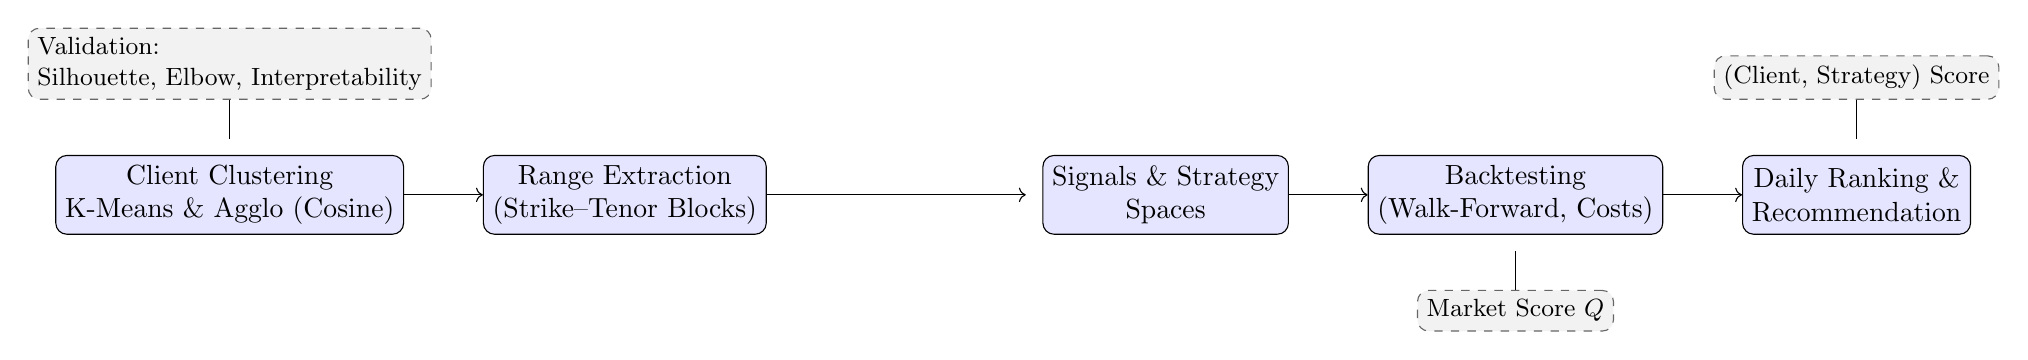
\begin{tikzpicture}[node distance=1cm]
\tikzstyle{box} = [rectangle, draw=black, rounded corners, minimum height=1cm, minimum width=1.7cm, align=center, fill=blue!10]
\tikzstyle{note} = [rectangle, draw=black!60, dashed, rounded corners, fill=gray!10, align=left, font=\small]

% Part I
\node[box] (cluster) {Client Clustering\\K-Means \& Agglo (Cosine)};
\node[box, right=of cluster] (ranges) {Range Extraction\\(Strike--Tenor Blocks)};

% Part II main flow
\node[box, right=3.5cm of ranges] (signals) {Signals \& Strategy\\Spaces};
\node[box, right=of signals] (bt) {Backtesting\\(Walk-Forward, Costs)};
\node[box, right=of bt] (reco) {Daily Ranking \&\\Recommendation};

% Arrows Part I to Part II
\draw[->] (cluster) -- (ranges);
\draw[->, shorten >=6pt] (ranges.east) -- ++(0.8,0) |- (signals.west);
\draw[->] (signals) -- (bt);
\draw[->] (bt) -- (reco);

% Notes
\node[note, above=7mm of cluster] (val) {Validation:\\Silhouette, Elbow, Interpretability};
\draw[-] (val.south) -- ([yshift=2mm]cluster.north);

\node[note, below=7mm of bt] (metrics) {Market Score $Q$};
\draw[-] (metrics.north) -- ([yshift=-2mm]bt.south);



% Client + Strategy score feeding into final reco
\node[note, above=7mm of reco] (cscore) {(Client, Strategy) Score};
\draw[-] (cscore.south) -- ([yshift=2mm]reco.north);

\end{tikzpicture}%
}
\caption{Two-part pipeline: client profiling (left) and strategy \& recommendation engine (right). 
Backtesting relies on performance metrics (core + market score $Q$), and the final recommendation 
combines these with client-specific strategy scores.}
\label{fig:pipeline}
\end{figure}










\section{Client Representation and Clustering}

\subsection{Feature construction}

Each client \(c\) is represented by a feature vector 
\[
    \mathbf{x}_c = (x_{c,1}, x_{c,2}, \dots, x_{c,p}),
\]
where the components summarize the client’s trading behavior across products, underlyings, maturities, and risk exposures. The features used are:

\begin{itemize}

    \item \textbf{Strategy--side proportions:} 
    For each category $s$ of \texttt{STRATEGY\_SIDE}, the proportion of client $c$'s notional allocated 
    to $s$ is defined as
    \[
        \text{Prop}_{c,s} \;=\; 
        \frac{\sum_{i \in \mathcal{T}_{c,s}} \text{Notional}_{i}}
             {\sum_{i \in \mathcal{T}_{c}} \text{Notional}_{i}},
    \]
    where $\mathcal{T}_{c,s}$ is the set of trades of client $c$ with strategy-side label $s$, 
    and $\mathcal{T}_{c}$ is the set of all trades of client $c$. 
    This ensures that both direction (buy/sell) and strategy type are reflected in the client 
    representation, except for spreads and strangles where directionality is already 
    embedded in the strategy label.


    \item \textbf{Underlying type proportions:} defined analogously, distinguishing between index and single-stock underlyings.

    \item \textbf{Number of legs proportions:} share of single-leg vs multi-leg trades, defined analogously as the previous notional proportions.

    \item \textbf{Entropy measures:} for each categorical dimension (strategy-side, underlying type, number of legs), an entropy score is computed as
    \[
        H_c = - \sum_{j} p_{c,j} \log p_{c,j},
    \]
    where \(p_{c,j}\) is the notional share of client \(c\) allocated to category \(j\). A higher entropy indicates greater diversification across categories.

    \item \textbf{Weighted means and standard deviations:} for continuous variables such as booked implied volatility, delta dollar, vega dollar, gamma dollar, strike percentage, maturity width, strike width and maturity (in business days), client-level statistics are computed as notional-weighted averages. For example, for strike percentage:
    \[
        \text{MeanStrike\%}_c = \sum_{i \in \mathcal{T}_c} w_{c,i} \cdot \text{Strike\%}_{i}, 
        \quad \text{with } w_{c,i} = \frac{\text{Notional}_i}{\sum_{j \in \mathcal{T}_c} \text{Notional}_j}.
    \]
    A weighted standard deviation is defined analogously.

    \item \textbf{Trading activity measures:} number of active months, mean number of trades per month, total notional, and mean notional per trade.
\end{itemize}

The resulting feature vector provides a comprehensive representation of each client’s trading style, balancing categorical distributions (strategy, tenor, underlying), statistical moments of continuous characteristics (volatility, Greeks, strike), and activity-level indicators.


\subsection{Clustering methodology}

Once feature vectors are constructed, they are standardized to have zero mean and unit variance in order to remove scale effects. Two clustering approaches are then applied:

\paragraph{K-means clustering.}
K-means partitions the set of clients into \(K\) clusters by minimizing the within-cluster variance:
\[
    \min_{\{C_1, \dots, C_K\}} \sum_{k=1}^K \sum_{c \in C_k} \lVert \mathbf{x}_c - \boldsymbol{\mu}_k \rVert_2^2,
\]
where \(\boldsymbol{\mu}_k\) is the centroid of cluster \(C_k\). The algorithm iterates between (i) assigning each client to the nearest centroid, and (ii) updating centroids as the mean of assigned points, until convergence. The optimal number of clusters \(K\) is selected using the elbow method and silhouette scores.

\paragraph{Agglomerative clustering with cosine similarity.}  
To complement K-means, we also implement hierarchical agglomerative clustering, a bottom-up method that builds a hierarchy of nested clusters. The procedure begins with each client forming its own singleton cluster. At each iteration, the algorithm identifies the two clusters with the smallest distance and merges them, continuing until all clients belong to a single cluster. Clusters are merged iteratively until a single tree (dendrogram) is formed, where the vertical axis encodes the distance at which clusters are joined; cutting this tree at a chosen height produces the final groups.


The dissimilarity between two clients $i$ and $j$ is measured using \textbf{cosine distance}, defined as  
\[
    d(\mathbf{x}_i, \mathbf{x}_j) \;=\; 1 - \frac{\mathbf{x}_i \cdot \mathbf{x}_j}{\lVert \mathbf{x}_i \rVert \, \lVert \mathbf{x}_j \rVert},
\]  
where $\mathbf{x}_i$ and $\mathbf{x}_j$ denote the feature vectors of clients $i$ and $j$. Cosine distance captures angular differences, meaning it compares the \emph{composition} of strategy-side profiles rather than their absolute magnitudes. For example, two clients with the same relative mix of bull and bear spreads, but operating at different overall scales, will still be considered close under this metric.

When extending distance to clusters $C_p$ and $C_q$ containing multiple clients, we adopt the \textbf{average linkage} criterion:  
\[
    d(C_p, C_q) \;=\; \frac{1}{|C_p|\,|C_q|} \sum_{i \in C_p} \sum_{j \in C_q} d(\mathbf{x}_i, \mathbf{x}_j),
\]  
so the inter-cluster distance is simply the mean of all pairwise distances between their members. This linkage scheme balances the extremes of single linkage (which can form long chains) and complete linkage (which enforces very compact clusters), and generally produces well-balanced groups.  

The algorithm can be summarized as follows:  
\begin{enumerate}
    \item Initialize each client as its own cluster.  
    \item Compute all pairwise distances using cosine distance, to build the distance matrix.  
    \item Merge the two clusters with minimum distance.  
    \item Update the distance matrix according to the linkage criterion.  
    \item Repeat steps 3--4 until only one cluster remains.  
    \item Cut the dendrogram at a predefined threshold to obtain the final partition.  
\end{enumerate}

As an illustration, suppose clients $A$ and $B$ have cosine distance $d(A,B) = 0.2$, the smallest among all pairs. They are merged into a cluster $\{A,B\}$. The distance between this new cluster and another client $C$ is then computed as  
\[
    d(\{A,B\}, C) \;=\; \tfrac{1}{2}\big(d(A,C) + d(B,C)\big).
\]  
Iterating this process yields a hierarchical tree. By setting a distance cutoff (for instance $d=0.4$, corresponding to at least $60\%$ cosine similarity), we obtain the final groups of clients with similar trading profiles.

\paragraph{Cluster validation.}
Cluster quality is assessed using both internal and external criteria. Internally, silhouette scores quantify the separation between clusters and help identify a suitable number of groups. Externally, interpretability is checked by examining whether clusters align with economically meaningful profiles (e.g., volatility sellers vs.\ directional traders).  

In practice, we retain \textbf{K-means clustering} as the primary method used throughout the remainder of this report, since it provides stable partitions and is well suited for large datasets. \textbf{Agglomerative clustering with cosine similarity} is employed as a robustness check: by comparing dendrogram-based groupings with the K-means results, we verify that observed client structures are not an artifact of the chosen algorithm.


\section{Identification of Strategy Ranges}

After clustering clients, the next step is to extract the most representative product ranges within each cluster. The objective is to identify contiguous regions of trading activity in the strike–tenor space, where clients concentrate their notional exposures. 

\subsection{Construction of notional grids}

For each cluster \(C_k\), and for each product defined by the pair 
\((\texttt{STRATEGY\_TYPE}, \texttt{UNDERLYING\_INSTRUMENT\_TYPE})\), a notional grid is 
constructed to capture the distribution of trading activity across strike, maturity, and, 
where relevant, structural dimensions of multi-leg products.

Each cell stores the \emph{within-product, within-cluster} notional share, ensuring product mixes are comparable across clusters.


The grid specification depends 
on the product type:

\begin{itemize}
    \item \textbf{Calls, Puts, and Straddles:} represented on a two-dimensional grid 
    where the rows correspond to \textbf{tenor bins} (e.g.<1w, 1w, 2w, 3w, 1m, 2m…) and the columns correspond to \textbf{strike percentage bins} (e.g. 40–50\%, 90–95\%, …).

    \item \textbf{Strangles and Vertical Spreads (Bull/Bear Call/Put):} represented on a 
    three-dimensional grid with axes \emph{tenor bin}, \emph{strike percentage bin}, and 
    \texttt{strike\_width}.  
    \item \textbf{Calendar Spreads (Bull/Bear Call/Put):} represented on a 
    three-dimensional grid with axes \emph{tenor bin}, \emph{strike percentage bin}, and 
    \texttt{maturity\_width}.  
    \item \textbf{Diagonal spreads:} excluded from the present analysis.  
\end{itemize}

Each cell \((t, s)\) or \((t, s, w)\) of the grid records the notional proportion of trades of the 
product in cluster \(C_k\) falling into tenor bin \(t\), strike bin \(s\), and width bin \(w\), 
normalized by the total notional of that product in cluster \(C_k\). For example, in the 
two-dimensional case the cell value is defined as
\[
    P_{k}(t,s) = 
    \frac{\sum_{i \in \mathcal{T}_{C_k}(t,s)} \text{Notional}_{i}}
         {\sum_{i \in \mathcal{T}_{C_k}^{\text{prod}}} \text{Notional}_{i}},
\]
where \(\mathcal{T}_{C_k}(t,s)\) denotes the set of trades of the product in cluster \(C_k\) whose 
maturity falls in tenor bin \(t\) and strike lies in strike bin \(s\), and 
\(\mathcal{T}_{C_k}^{\text{prod}}\) is the set of all trades of that product in cluster \(C_k\). 
In the three-dimensional case, the formula is extended with an additional dimension, either 
\texttt{strike\_width} or \texttt{maturity\_width}, depending on the product.

\subsection{Range extraction via region growing}\label{subsec:range_extraction}

To extract contiguous areas of concentrated client activity, a region-growing algorithm is applied 
to each grid:

\begin{enumerate}
    \item \textbf{Seed selection:} select the cell \((t^\ast, s^\ast)\) or \((t^\ast, s^\ast, w^\ast)\) with the highest notional proportion \(P_{k}(t,s)\) or \(P_{k}(t,s,w)\) exceeding a minimum threshold~$\theta$ as the starting point of the first range.  
\item \textbf{Neighborhood expansion:} 
examine the neighboring cells around the current range. In two dimensions, each cell has up to 
eight neighbors (up, down, left, right, and diagonals). In three dimensions, each cell has up to 
26 neighbors (including adjacencies along all three axes and diagonals). If a neighboring cell 
has a notional proportion above the fixed threshold~$\theta$, it is included in the range. 
If it falls below~$\theta$, the expansion in that direction stops.  

\item \textbf{Iteration:} 
continue the expansion until no additional neighbors exceed the threshold. The resulting connected 
region defines a strike--tenor (or strike--tenor--width) range.  

\item \textbf{Multiple ranges:} 
once the first range is established, search the grid for other unvisited cells with 
proportion \(P_{k}(t,s)\) or \(P_{k}(t,s,w)\) above~$\theta$. Each such cell becomes the seed of a new range, 
and the expansion procedure is repeated until no qualifying cells remain.  

\end{enumerate}

\subsection{Output and interpretation}

The procedure yields, for each cluster and product type, one or several ranges characterized by:
\begin{itemize}
    \item the strategy type and underlying instrument type,  
    \item a contiguous block of tenor bins and strike bins,  
    \item and, when applicable, a contiguous block of \texttt{strike\_width} or \texttt{maturity\_width}.  
\end{itemize}

These ranges capture the localized patterns of client demand within the strike--tenor space, 
and, for multi-leg products, along the additional dimension of strike or maturity width. 
For example, a cluster might be characterized by European Calls on indices with strikes 
between 40--50\% and 90--95\% of spot and tenors between 1M and 3M. Another cluster might 
concentrate in bear call spreads with strike widths of 5--10\% and maturities around 6M. 
Yet another may exhibit demand for calendar spreads centered at the 100\% strike with 
maturity differences of 1--3 months. These ranges serve as structural inputs for the subsequent 
stage of historical trade generation, signal design, and backtesting.




\section{Underlying Selection and Historical Trade Generation}

Once strategy ranges have been identified for each cluster, the next step is to generate historical trade datasets that replicate the products most representative of client activity. These datasets serve as the basis for signal application and backtesting.

\subsection{Selection of relevant ranges and underlyings}

For each cluster \(C_k\) and each product defined by \((\texttt{STRATEGY\_TYPE}, \texttt{UNDERLYING\_INSTRUMENT\_TYPE})\), the ranges extracted in the previous step are filtered according to their notional importance. Only ranges accounting for at least 10\% of the cluster’s total notional are retained:
\[
    \text{Range } r \text{ is selected if } 
    \frac{\sum_{i \in \mathcal{T}_{C_k}(r)} \text{Notional}_i}{\sum_{i \in \mathcal{T}_{C_k}} \text{Notional}_i} \geq 0.10,
\]
where \(\mathcal{T}_{C_k}(r)\) is the set of trades in cluster \(C_k\) that fall within range \(r\).

For each selected range, the top three underlyings are identified by traded notional:
\[
    U_{k,r} = \arg\max_{U \in \mathcal{U}} \ \sum_{i \in \mathcal{T}_{C_k}(r,U)} \text{Notional}_i,
\]
where \(\mathcal{T}_{C_k}(r,U)\) denotes trades in range \(r\) with underlying \(U\). This ensures that the generated trades are anchored to the most representative instruments.


\subsection{Computation of trade-level PnL and Greeks}

A trade is defined by its underlying $U$, entry date $t_0$, expiry $T$, strike $K$, and (if applicable) structure $a$. Let $V(\tau;K,T,U)$ denote the \emph{fair value} (FV) of the option or structure at time $\tau$ (marked from market mid quotes or a pricing model consistent with implied volatility).

For a long position entered at $t_0$ and exited at $t_1\le T$, the trade-level PnL is
\[
\text{PnL}(t_0\!\to\!t_1) \;=\; V(t_1;K,T,U)\;-\;V(t_0;K,T,U).
\]
If the position is held to expiry, $t_1=T$ and $V(T;K,T,U)$ equals intrinsic value (e.g., $(S_T-K)^+$ for a call), up to carry/settlement conventions. For multi-leg structures, $V(\cdot)$ is the \emph{net} FV (long legs positive, short legs negative); the same formula applies.

\paragraph{Example (range call at 107.5\%).}
For a 1M European call initiated on $t_0$ with strike $K=1.075\,S_{t_0}$ and expiry $T=t_0+1\text{M}$, the realized PnL upon exit $t_1\le T$ is
\[
\text{PnL}(t_0\!\to\!t_1) \;=\; V(t_1;1.075\,S_{t_0},T,U)\;-\;V(t_0;1.075\,S_{t_0},T,U).
\]
Daily PnL increments used for performance metrics are $\Delta \text{PnL}(\tau)=V(\tau;K,T,U)-V(\tau\!-\!1;K,T,U)$ for $\tau\in(t_0,t_1]$. When reporting return-style metrics, we also use the premium-normalized figure
\[
r_{\text{trade}}(t_0\!\to\!t_1)\;=\;\frac{\text{PnL}(t_0\!\to\!t_1)}{\big|V(t_0;K,T,U)\big|}.
\]

\paragraph{Greeks.}
Risk sensitivities are computed on each business day $\tau\in[t_0,t_1]$ from the same pricing setup:
\[
\Delta(\tau)=\frac{\partial V}{\partial S}(\tau),\qquad
\Gamma(\tau)=\frac{\partial^2 V}{\partial S^2}(\tau),\qquad
\nu(\tau)=\frac{\partial V}{\partial \sigma}(\tau),
\]
with netting across legs for spreads/combos.

 TO BE REVISED 
 
The output of this stage is a comprehensive dataset of hypothetical trades for each cluster–range–underlying triplet, including their daily PnL and Greek trajectories. This dataset forms the input for the signal design and backtesting stages.



 TO BE REMOVED OR INCLUDED TO LATER PARAGRAPHS


\section{Signal Design: Theoretical Background}

In Part~II of the pipeline (Strategy \& Recommendation Engine), market observables are transformed into rule-based \emph{strategy spaces}. The strategy spaces employed fall into three broad categories—\textbf{momentum}, \textbf{volatility}, and \textbf{mean-reversion}—each grounded in the academic literature and widely applied in equity and derivative markets. Each space is defined by (i) a set of signals that characterize a regime, (ii) an \emph{action universe} of eligible option structures, and (iii) exit/adjust rules. This section develops the \emph{theoretical} building blocks of these signals and later uses them to specify the spaces and backtest them systematically on large underlying universes. We denote by $S_t$ the underlying spot at date $t$, by $r_t=\log(S_t/S_{t-1})$ the daily log-return, and by $\sigma^{\text{IV}}_{\tau,t}$ the at-the-money (ATM) implied volatility of maturity $\tau$ observed at $t$.





before explaining how they are combined into strategy rules and illustrated with concrete examples.


\subsection{Momentum indicators and strategies}

Momentum is one of the most robust predictors of returns across asset classes \citep{jegadeesh1993returns, moskowitz2012time}. In options, momentum signals are often combined with filters such as the Relative Strength Index (RSI) or the Average Directional Index (ADX) to confirm trend direction and strength.

\paragraph{Time-series momentum.}  
With a lookback horizon of $L$ months and an optional skip parameter, momentum is defined as:
\[
\text{Mom}_{t}^{(L,\text{skip})}
= \sum_{j=\text{skip}}^{L+\text{skip}-1} r_{t-j}
= \log\!\left(\frac{S_{t-\text{skip}}}{S_{t-L-\text{skip}}}\right).
\]
A positive value indicates an uptrend, a negative value a downtrend. In practice, the ``$12\!-\!1$'' specification (12 months excluding the most recent) has been shown to capture persistent trends in equities \citep{moskowitz2012time}.

\paragraph{Relative Strength Index (RSI).}  
The RSI \citep{wilder1978new} is a bounded oscillator that measures the magnitude of recent gains relative to losses. With a smoothing window $n$:
\[
g_t=\max(S_t-S_{t-1},0), \quad \ell_t=\max(S_{t-1}-S_t,0),
\]
\[
\overline{g}_t=\alpha g_t+(1-\alpha)\overline{g}_{t-1},\quad 
\overline{\ell}_t=\alpha \ell_t+(1-\alpha)\overline{\ell}_{t-1}, \quad \alpha=\tfrac{1}{n},
\]
\[
\text{RS}_t=\frac{\overline{g}_t}{\overline{\ell}_t}, \qquad \text{RSI}_t=100-\frac{100}{1+\text{RS}_t}.
\]
Values above 50 typically confirm bullish momentum, while values below 50 indicate bearish regimes \citep{brock1992simple}.

\paragraph{Average Directional Index (ADX).}  
The ADX \citep{wilder1978new} measures the strength of a trend regardless of its direction. First, define the True Range:
\[
\text{TR}_t=\max\{H_t-L_t,\ |H_t-C_{t-1}|,\ |L_t-C_{t-1}|\},
\]
where $H_t$, $L_t$, and $C_t$ are respectively the high, low, and close prices at time $t$. Directional movements are then:
\[
+DM_t=\max(H_t-H_{t-1},0) \ \text{if } H_t-H_{t-1} > L_{t-1}-L_t,\ \text{else } 0,
\]
\[
-DM_t=\max(L_{t-1}-L_t,0) \ \text{if } L_{t-1}-L_t > H_t-H_{t-1},\ \text{else } 0.
\]

To smooth these series, we use \textit{Wilder’s smoothing}, which is an exponential moving average with coefficient $\alpha=\tfrac{1}{n}$:
\[
X^{(n)}_t=\alpha X_t+(1-\alpha)X^{(n)}_{t-1}, \qquad \alpha=\frac{1}{n},
\]
applied to $X\in\{+DM, -DM, \text{TR}\}$, yielding $+DM^{(n)}_t$, $-DM^{(n)}_t$, and $\text{TR}^{(n)}_t$.

Directional indicators are then defined as:
\[
+DI_t=100\cdot\frac{+DM^{(n)}_t}{\text{TR}^{(n)}_t}, \qquad
-DI_t=100\cdot\frac{-DM^{(n)}_t}{\text{TR}^{(n)}_t}.
\]
The directional index is:
\[
\text{DX}_t=100\cdot\frac{|+DI_t-(-DI_t)|}{+DI_t+(-DI_t)}.
\]

Finally, the ADX is obtained as the Wilder-smoothed moving average of $\text{DX}_t$. In practice, $\text{ADX}<20$ indicates a weak or range-bound market, $20\!-\!25$ signals the emergence of a trend, and $\text{ADX}>25$ is taken as confirmation of a strong trend.


\subsection{Volatility indicators and strategies}

Implied volatility surfaces contain rich information about expected risks and investor demand. Several indicators are extracted from the level, slope, and difference between implied and realized volatility.

\paragraph{Implied vs realized volatility (variance risk premium).}  
Realized volatility over $h$ days is:
\[
\sigma^{\text{RV}}_{h,t}=\sqrt{\frac{252}{h}\sum_{j=1}^h r_{t-j}^2}.
\]
The variance risk premium is:
\[
\Delta^{\text{VRP}}_{\tau,h,t} = \left(\sigma^{\text{IV}}_{\tau,t}\right)^2 - \left(\sigma^{\text{RV}}_{h,t}\right)^2.
\]
A positive VRP reflects that implied variance systematically exceeds realized variance, consistent with the literature on volatility risk premia \citep{carr2001empirical, bollerslev2009volatility}. ``IV normal/low'' conditions are captured by standardized $z$-scores of $\sigma^{\text{IV}}_{\tau,t}$.


\paragraph{Implied-volatility level (percentile rank, ``IVRank'').}
Rather than standardizing $\sigma^{\text{IV}}_{\tau,t}$ with a $z$-score, we use a rolling
\emph{percentile rank} that compares today’s IV to its own recent history. For a maturity
$\tau$ (in practice $\tau=1$M, ATM) and a rolling window of $W$ trading days, define the
empirical CDF $\widehat{F}^{(W)}_{\tau,t}(\cdot)$ of
$\{\sigma^{\text{IV}}_{\tau,t-j}\}_{j=1}^{W}$. The IV rank is
\[
\text{IVRank}_{\tau,t}^{(W)} \;=\; 100 \times
\widehat{F}^{(W)}_{\tau,t}\!\big(\sigma^{\text{IV}}_{\tau,t}\big)
\;\in\;[0,100].
\]
Operationally, we compute $\text{IVRank}_{1\text{M},t}^{(W)}$ using ATM 1M IV and
$W\in\{252,504\}$ depending on the horizon. Low values (e.g., $\le 30$th percentile)
indicate \emph{historically cheap} implied volatility; high values (e.g., $\ge 70$th) indicate
\emph{historically rich} IV. This ranking is robust to slow level shifts and facilitates
rule-based gating across strategy spaces: low IV percentiles support long-convexity
structures (e.g., calls, long-gamma), whereas high percentiles favor premium-selling or
spread constructions that offset rich option prices. For reference, if a normal approximation
is acceptable, the percentile $p$ corresponds to a $z$-score via $p\approx \Phi(z)$, but we
use the empirical rank in backtests.


\paragraph{Skew.}  
The slope of implied volatility across strikes (smile asymmetry) is a proxy for downside protection demand \citep{bollen2004does}. Around ATM:
\[
\text{Skew}_{\tau,t} \approx \frac{\sigma^{\text{IV}}_{\tau,t}(K_2)-\sigma^{\text{IV}}_{\tau,t}(K_1)}{(K_2-K_1)/S_t}, \quad K_1<K_{ATM}<K_2.
\]
High skew signals expensive puts; mild skew corresponds to near-symmetric smiles.

\paragraph{Term structure.}  
The slope between two maturities $\tau_1<\tau_2$ is:
\[
\text{TS}_t=\sigma^{\text{IV}}_{\tau_2,t}-\sigma^{\text{IV}}_{\tau_1,t}.
\]
Positive slopes (contango) reflect increasing forward uncertainty; negative slopes (backwardation) often occur in stressed markets \citep{christoffersen2009shape}.

\subsection{Mean-reversion and compression indicators}

While momentum and volatility indicators capture directional and convex exposures, mean-reversion signals exploit short-term overreaction and volatility clustering.

\paragraph{Bollinger bands.}  
With moving average $m_t=\text{SMA}_n(S)_t$ and rolling standard deviation $s_t$:
\[
\text{UB}_t=m_t+ks_t, \quad \text{LB}_t=m_t-ks_t.
\]
The band width is
\[
\text{BW}_t=\frac{\text{UB}_t-\text{LB}_t}{m_t}.
\]
Low $\text{BW}_t$ (below a historical percentile) indicates volatility compression, often preceding large moves (``squeezes''). Conversely, touches of UB or LB combined with RSI extremes are classic mean-reversion signals \citep{brock1992simple}.

\subsection{Summary}

The combination of these indicators allows the classification of market regimes into three archetypes: (i) strong directional trends confirmed by RSI and ADX, (ii) volatility dislocations signaled by high VRP, skew, or unusual term-structure slopes, and (iii) mean-reverting or compression phases flagged by Bollinger bands. In the next subsection, these theoretical signals are operationalized into specific option structures (e.g., call spreads, put spreads, straddles), aligned with the recommendation framework.

\section{From Signals to Strategies (Strategy Spaces \& Action Universes)}
\label{sec:spaces_action}

ADD OTHER MOMENTUM STRATEGIES FROM THE TABLE ETC 


Once momentum, volatility, and mean-reversion indicators are computed, they are grouped into \emph{strategy spaces}. A strategy space specifies:
\begin{enumerate}
    \item \textbf{Activation (signals/regime):} logical gates that must all hold for entry.
    \item \textbf{Action universe:} the menu of option structures permissible under this regime (e.g., calls, verticals, calendars) with construction guides (DTE bands, strike grids, widths).
    \item \textbf{Exit/adjust:} earliest-exit rules (signal invalidation, technical breaks) and profit/risk targets.
\end{enumerate}

The mapping follows the desk’s practice and the specification table used operationally (signal state $\rightarrow$ direction/vol view $\rightarrow$ recommended structures $\rightarrow$ construction guide $\rightarrow$ exit/adjust).
\\

We begin with the following \emph{strategy spaces} as the initial set; they will be expanded progressively as empirical evidence and desk feedback accumulate. Each space specifies (i) activation via signal gating, (ii) a backtest \emph{action universe} (structures and grids), and (iii) exit/adjust rules.

\paragraph{Strategy space: Momentum (bullish).}
\textbf{Activation:} $\mathrm{ROC}_{L}(t)>0$, $S_t>\mathrm{SMA}_{50}(t)>\mathrm{SMA}_{200}(t)$, $\mathrm{ADX}_{n}(t)>\tau_{ADX}$, $\text{IVRank}^{(252)}_{1\mathrm{M},t} \le 40$\footnote{%
$\text{IVRank}^{(W)}$ is the rolling percentile of ATM 1M implied volatility over a window $W$.}
. \\[2pt]
\textbf{Reasoning:} Positive returns over the lookback, aligned moving averages, and $\mathrm{ADX}$ above threshold indicate a persistent, directional uptrend with adequate trend strength. A non-positive IV $z$-score suggests benign pricing of convexity. In such regimes, \emph{long-delta, long-gamma} structures benefit from continuation while capping downside risk to the paid premium. Spreads retain convexity but reduce premium outlay by selling part of the upside where marginal convexity is less valuable. \\[2pt]
\textbf{Action universe (backtest):}
\begin{itemize}
    \item \emph{Long Call:} $K \in \{85\%,90\%,95\%,100\%,105\%,110\%\}$,\quad
    $T \in \{1\text{M},2\text{M},3\text{M},4\text{M},5\text{M},6\text{M},7\text{M},8\text{M},9\text{M},10\text{M},11\text{M},12\text{M},24\text{M}\}$.
    \item \emph{Bull Call Spread:} $K_1 \in \{85\%,90\%,95\%,100\%,105\%\}$,\; width $w \in \{3\%,5\%,7\%,10\%\}$,\; $K_2=K_1+w$;\;
    $T$ on the same tenor grid.
\end{itemize}
\textbf{Exit/adjust:} take profits at 50--75\% of max; exit on $S_t < \mathrm{SMA}_{50}(t)$, or $\mathrm{SMA}_{50}\le\mathrm{SMA}_{200}$, or if trend filters (RSI/ADX) break.

\paragraph{Strategy space: Volatility dislocation (downside skew).}
\textbf{Activation:} elevated put skew and positive VRP; momentum neutral/bearish. \\[2pt]
\textbf{Reasoning:} Rich downside skew implies OTM puts are expensive relative to ATM; a positive variance risk premium indicates implied variance exceeds realized on average. With non-bullish momentum, downside hedging demand is high but costly. \emph{Debit put spreads} monetize the rich wing by selling an even further OTM put to partially finance the long put. \emph{Put calendars} sell nearer-term (richer) implied variance against longer-dated exposure, aligning with positive VRP and term-structure carry while keeping a downside bias. \\[2pt]
\textbf{Action universe (backtest):}
\begin{itemize}
    \item \emph{Bear Put Debit Spread:} long strike $K_L \in \{90\%,95\%,100\%\}$,\; width $w \in \{3\%,5\%,7\%,10\%\}$,\; short strike $K_S=K_L-w$;\;
    $T \in \{1\text{M},\dots,12\text{M},24\text{M}\}$.
    \item \emph{Put Calendar (near ATM):} $K \in \{95\%,100\%\}$,\; front/back maturities $(T_f, T_b)$ from
    $\{(1,3),(1,6),(2,6),(3,6),(3,9),(3,12),(6,12),(6,24)\}$ months.
\end{itemize}
\textbf{Exit/adjust:} take profits when the debit spread reaches 50--75\% of its maximum value; for calendars, exit on normalization of skew/VRP or if spot closes back above the short strike.

\paragraph{Strategy space: Compression/breakout.}
\textbf{Activation:} low Bollinger bandwidth, ADX $<20$, momentum neutral. \\[2pt]
\textbf{Reasoning:} Narrow bands with weak trend indicate volatility compression and potential for abrupt breaks. \emph{Long-gamma} structures (straddles/strangles) benefit from either-direction moves and IV expansion. \emph{Double calendars} position for a pickup in near-term realized volatility and/or favorable roll of term structure around ATM, while moderating directional exposure. \\[2pt]
\textbf{Action universe (backtest):}
\begin{itemize}
    \item \emph{Long Straddle (ATM):} $K=100\%$,\; $T \in \{1\text{M},\dots,12\text{M},24\text{M}\}$.
    \item \emph{Long Strangle (symmetric wings):} $(K_{\text{put}},K_{\text{call}})=(100\%-b,\ 100\%+b)$ with 
    $b \in \{3\%,5\%,7\%,10\%\}$,\; $T$ on the same tenor grid.
    \item \emph{Double Calendar (ATM):} $K=100\%$,\; pairs $(T_f,T_b)$ from 
    $\{(1,3),(1,6),(2,6),(3,6),(3,9),(3,12),(6,12),(6,24)\}$ months.
\end{itemize}
\textbf{Exit/adjust:} exit on IV pop accompanied by directional break; use time stops to avoid prolonged decay if no breakout occurs.



The universes above will then be backtested over the full top-100 underlying set using strike and tenor from the action universe; \textbf{no cluster or client filters are applied during backtests}. Client profiling from Part~I is incorporated \emph{after} backtesting via a compatibility score to prioritize which clients are most likely to engage with each active $(\text{strategy space},\ \text{underlying},\ \text{structure})$.

\noindent\emph{Backtest } For \emph{each} strategy space and its action universe, we run a grid backtest across the top-100 underlyings and the tenor/strike (or width) grids specified above. For every tuple
\[
(s,\ \theta,\ U,\ a,\ T,\ K\ \text{or}\ w),
\]
\emph{where} $s$ is the strategy space, $\theta$ the signal parameters, $U$ the underlying, $a$ the option structure, $T$ the maturity (or $(T_f,T_b)$ for calendars), and $K$ (or $w$) the strike choice(s) relevant to $a$, we compute and \emph{store} in a model table the key performance metrics
\[
\{\text{Sharpe},\ \text{Sortino},\ \text{Max Drawdown},\ \text{Hit Rate},\ \text{Avg Trade PnL},\ \text{Turnover},\ \text{Exposure}\},
\]
along with costs and date ranges. This table is later queried by the daily engine to score active signals and by the client-profiling layer to rank recommendations.


\medskip
In all spaces, activation uses logical gating (all conditions must hold). The next section details how these spaces are \emph{systematically backtested} across underlyings and parameter grids, and how their results populate a persistent \emph{model store} used by the daily engine.

\section{Backtesting Framework and Model Store}
\label{sec:bt_modelstore}

For each strategy space $s$ and each of its signal groups $g$ \emph{as presented in Section~\ref{sec:spaces_action}}, we specify a parameter tuple $\theta_{s,g}$ (e.g., for Momentum–Bullish: lookback $L$, ADX window $n_{\mathrm{ADX}}$ and threshold $\tau_{\!ADX}$, IVRank window $W$ and percentile $p^{\text{IVR}}$, and SMA lengths). For every $(s,g,\theta_{s,g})$ we run a grid backtest across the \textbf{top 100 underlyings}. The \emph{action universes} in Section~\ref{sec:spaces_action} determine the option structures $a$ and the grids over strikes $K$, tenors $T$ (or widths $w$) instantiated whenever the $(s,g,\theta_{s,g})$ activation gate is true. Results are persisted for downstream ranking and recommendation.

\subsection{Run-time backtest routine and results persistence}

When the tool is run on a business date $t$, it evaluates all $(s,g,\theta_{s,g})$ across the top 100 underlyings. For each underlying $U$, whenever the activation gate is true, the engine instantiates trades for every admissible option structure $a$ in the action universe of $s$ (with the prescribed $K$, $w$, $T$ grids) and simulates them using the P\&L/Greeks definitions given earlier (fair value at exit minus fair value at entry, marked to end-of-day).

\paragraph{Historical window and date generation.}
Each run backtests over a configurable historical window ending at $t$ (e.g., January 2016 to $t$). For every business day $u$ in that window on which the gate holds, trades are instantiated on $u$ with expiries mapped from the tenor grid to listed maturities by market convention. For equity monthly expiries we use the third-Friday rule: for a tenor of $d$ months,
\[
T_d(u)\;=\;\min\{\ \tau\in\mathcal{C}\ :\ \tau\ge u+d\text{ months},\ \tau\ \text{is the 3rd Friday}\ \}.
\]
For calendars/double calendars, expiry pairs $(T_{d_f}(u),T_{d_b}(u))$ are formed from the allowed $(d_f,d_b)$ combinations in the action universe. Each trade is carried from entry $t_0=u$ to the earliest exit (signal invalidation, SMA break, time stop) or to expiry; daily increments $\Delta\mathrm{PnL}(\tau)$ are built from end-of-day fair values.

\paragraph{What is stored.}
Every completed trade writes one row to the results table keyed by
\[
(s,\ g,\ \theta_{s,g},\ U,\ a,\ T,\ K\ \text{or}\ w;\ \text{test\_from},\ \text{test\_to}),
\]
together with headline metrics: Sharpe, Sortino, Max Drawdown, Cumulative Return, Hit Rate, \textbf{Entry frequency (trades/year)}, Exposure, and costs. In parallel, a \emph{parameter-summary} view aggregates metrics per $(s,g,\theta_{s,g})$ across underlyings/structures (median across $U$ by default), yielding the compact “one line per parameter set” used downstream.

\paragraph{Illustration (per-underlying parameter–summary for Momentum–Bullish).}
Below we show three illustrative parameter tuples for the Momentum–Bullish group; the metrics are populated by the backtest. For each fixed parameter tuple $(s,g,\theta_{s,g})$, we report the headline metrics \emph{per underlying}, optionally including the option structure $a$ when the downstream recommendation is structure-specific:
\[
\theta_{s,g}=\big(L,\ n_{\mathrm{ADX}},\ \tau_{\!ADX},\ W,\ p^{\text{IVR}},\ n_{\text{SMA}}^{\text{short}}/n_{\text{SMA}}^{\text{long}}\big).
\]

\begin{table}[h]
\centering
\begin{tabular}{lcccccccccccccc}
\toprule
$s$ & $g$ & $U$ & $[\text{from},\text{to}]$ & $L$ & $n_{\mathrm{ADX}}$ & $\tau_{\!ADX}$ & $W$ & IVRank ($p^{\text{IVR}}$) & $n_{\text{SMA}}^{\text{short}}/n_{\text{SMA}}^{\text{long}}$ & $a$ & Sharpe & MaxDD & CumRet & \textbf{Entries/yr} \\
\midrule
Momentum & Bullish & MSFT & 2016--$t$ & 6M  & 14 & 25 & 252 & $\le 40$ & 50/200 & Bull Call Spr. & \emph{filled} & \emph{filled} & \emph{filled} & \emph{filled} \\
Momentum & Bullish & AMZN & 2016--$t$ & 6M  & 14 & 25 & 252 & $\le 40$ & 50/200 & Long Call      & \emph{filled} & \emph{filled} & \emph{filled} & \emph{filled} \\
Momentum & Bullish & AAPL & 2016--$t$ & 6M  & 14 & 25 & 252 & $\le 40$ & 50/200 & Bull Call Spr. & \emph{filled} & \emph{filled} & \emph{filled} & \emph{filled} \\
\vdots    & \vdots  & \vdots & \vdots  & \vdots & \vdots & \vdots & \vdots & \vdots & \vdots & \vdots & \vdots & \vdots & \vdots & \vdots \\
\bottomrule
\end{tabular}
\caption{Per-underlying parameter–summary on run date $t$: one row per underlying $U$ (and, if used, structure $a$) for a fixed $(s,g,\theta_{s,g})$, showing metrics needed for trade idea selection.}
\label{tab:param-summary-mom-bull-perU}
\end{table}

\paragraph{Parameter definitions (Momentum–Bullish).}
We use $\theta_{\text{Mom,Bull}}=\big(L,\ n_{\mathrm{ADX}},\ \tau_{\!ADX},\ W,\ p^{\text{IVR}},\ (n_{\text{SMA}}^{\text{short}},n_{\text{SMA}}^{\text{long}})\big)$ with:
\begin{itemize}
    \item $L$ — momentum lookback used in $\mathrm{ROC}_{L}(t)=S_t/S_{t-L}-1$;
    \item $n_{\mathrm{ADX}}$ — ADX window length (business days) for Wilder smoothing;
    \item $\tau_{\!ADX}$ — ADX activation threshold (trend strength);
    \item $W$ — window (trading days) for the ATM 1M IV percentile rank (IVRank);
    \item $p^{\text{IVR}}$ — IVRank gating percentile (activation if $\text{IVRank}^{(W)}_{1\mathrm{M},t}\le p^{\text{IVR}}$);
    \item $(n_{\text{SMA}}^{\text{short}},n_{\text{SMA}}^{\text{long}})$ — short/long moving-average lengths for the price filter.
\end{itemize}
\noindent\textit{Table column mapping:} $n_{\mathrm{ADX}}$ appears as its own column; SMA lengths appear as $n_{\text{SMA}}^{\text{short}}/n_{\text{SMA}}^{\text{long}}$.

\section{Candidate Selection and Ranking}
\label{sec:selection_ranking}

On run date $t$, the engine produces, for each strategy space $s$ and signal group $g$, a ranked list of underlyings $U$ (and optionally structures $a$) that satisfy both (i) \emph{today’s} activation gate and (ii) \emph{historical} quality conditions drawn from the model store.

\subsection{Eligibility and ranking metrics}
For each $(s,g)$ and underlying $U$, we require $\text{gate}_{s,g}(U,t)=1$ (signals in Section~\ref{sec:spaces_action} hold on $t$).

Next, we define multiple metrics that will be computed from the backtest for $(s,g,U)$ and used both to rank candidates and, where indicated, to enforce minimum/maximum thresholds.

\begin{itemize}
        \item \emph{Out-of-sample Sharpe} $\big(\mathrm{Sharpe}_{\text{OOS}}\big)$: ratio of the mean daily strategy return to its standard deviation, annualized (factor $\sqrt{252}$). Daily returns are built from the simulated P\&L series according to the P\&L definition in Section~\ref{sec:bt_modelstore}.
        \item \emph{Average trade P\&L} $(\mathrm{AvgTradePnL})$: arithmetic mean of end-to-end P\&L per trade over the backtest window,
        \[
        \mathrm{AvgTradePnL}=\frac{1}{N_{\text{trades}}}\sum_{i=1}^{N_{\text{trades}}}\mathrm{PnL}_i,
        \]
        with $\mathrm{PnL}_i=V(t_{1,i})-V(t_{0,i})$ for trade $i$ (fair value at exit minus fair value at entry, net of costs). Optionally, a normalized version per unit premium or notional can be reported for comparability across structures.
        
        \item \emph{Maximum drawdown} $(\mathrm{MaxDD})$: largest peak-to-trough loss of the cumulative P\&L curve,
        \[
        \mathrm{MaxDD} \;=\; \max_{t}\left(1-\frac{C_t}{\max_{s\le t} C_s}\right),
        \]
        with $C_t$ the cumulative value process.
        
        \item \emph{Drawdown duration}:
        average length (days) of drawdown spells on the cumulative value curve. If $(t_{\text{peak}}^j,t_{\text{recover}}^j)$
        indexes drawdown $j$ from the last peak to full recovery,
        \[
        \mathrm{DDur}=\frac{1}{J}\sum_{j=1}^{J}\big(t_{\text{recover}}^j-t_{\text{peak}}^j\big)
        \quad
        \text{(median can be used for robustness).}
        \]
        Penalizes long slump periods even when MaxDD is moderate.
        \item \emph{Hit rate} $(\mathrm{HitRate})$: fraction of trades with positive total P\&L,
        \[
        \mathrm{HitRate} \;=\; \frac{\#\{\mathrm{PnL}(t_0\!\to\!t_1)>0\}}{\#\{\text{trades}\}}.
        \]
        \item \emph{Entry frequency (trades/year)}: activation frequency,
        \[
        \mathrm{Entries/yr} \;=\; \frac{N_{\text{entries}}}{Y}, \qquad Y=\text{years in window}.
        \]
        \item \emph{Average implied volatility} $(\mathrm{IVAvg})$: level proxy based on the option surface; arithmetic mean of ATM (or fixed-$\Delta$) implied volatilities at 1M, 3M, and 1Y maturities.
        \item \emph{Average carry (IV vs RV)} $(\mathrm{CarryAvg})$: average \emph{Variance Risk Premium (VRP)} across horizons,
        \[
        \mathrm{VRP}_H \;=\; \mathrm{IV}_H^{\,2}-\mathrm{RV}_H^{\,2}, \qquad
        \mathrm{CarryAvg} \;=\; \tfrac{1}{3}\!\left(\mathrm{VRP}_{1\mathrm{M}}+\mathrm{VRP}_{3\mathrm{M}}+\mathrm{VRP}_{1\mathrm{Y}}\right),
        \] 
        where $\mathrm{RV}_H$ is realized volatility over horizon $H$ (e.g., $\mathrm{RV}_{1\mathrm{M}}=\sqrt{\tfrac{252}{h}\sum_{j=1}^{h} r_{t-j}^2}$ with $h\approx 20$ trading days).
        \item \emph{Upside skew (yesterday)} $\big(\mathrm{UpsideSkew}_{\text{yday}}\big)$: richness of the call wing at 1M on $t\!-\!1$,
        \[
        \mathrm{UpsideSkew}_{\text{yday}} \;=\; \sigma_{25\Delta\,\text{call},\,1\mathrm{M}}(t\!-\!1) \;-\; \sigma_{\mathrm{ATM},\,1\mathrm{M}}(t\!-\!1).
        \]
        \item \emph{Downside skew (yesterday)} $\big(\mathrm{DownsideSkew}_{\text{yday}}\big)$:
        richness of the put wing at 1M on $t\!-\!1$,
        \[
        \mathrm{DownsideSkew}_{\text{yday}}=\sigma_{25\Delta\,\text{put},\,1\mathrm{M}}(t\!-\!1)-\sigma_{\mathrm{ATM},\,1\mathrm{M}}(t\!-\!1).
        \]
        (Equivalently, one can use the $25\Delta$ risk reversal $\mathrm{RR}_{25}=\sigma_{25\Delta\,\text{call}}-\sigma_{25\Delta\,\text{put}}$;
        more negative $\mathrm{RR}_{25}$ means richer downside.)
        
        \item \emph{Cost per unit of protection at a shock} $\big(\mathrm{CP}_{\text{shock}}\big)$: 
        a hedge–efficiency ratio answering “how many dollars of premium do I pay today for one dollar of payout under a standardized downside scenario?” Formally,
        \[
        \mathrm{CP}_{\text{shock}}(a)
        =\frac{\text{Net Debit}(a)}{\max\!\big\{\,V^{\shock}(a)-V_0(a),\,\epsilon\big\}},
        \]
        where $V_0(a)$ is today’s fair value of structure $a$ (net of legs) \emph{computed with a consistent option–pricing model} (e.g., Black–Scholes using the observed IV surface, or market mids when available), and $V^{\shock}(a)$ is the \emph{same–model} re–pricing of $a$ under a common scenario:
        \[
        S\to S^{\shock}=S_0(1-\delta),\qquad 
        \sigma\to\sigma^{\shock}=\sigma_0+\Delta\sigma,\qquad
        t\to t+h.
        \]
        Here $\delta$ is the spot drop (e.g., $10\%$), $\Delta\sigma$ the implied-volatility up-shock, $h$ the horizon, and $\epsilon>0$ a small floor to avoid division by zero. \emph{Lower} $\mathrm{CP}_{\text{shock}}$ is better (more protection per dollar).
        \footnote{For comparability we fix the same protocol across candidates, e.g., $h=1$ month, spot shock $-10\%$, sticky-delta smile dynamics, and a positive vol up-shock, all applied consistently in the pricing model.}
        
        
        \item \emph{Stress P\&L at 5\%} $\big(\mathrm{StressPnL}_{5\%}\big)$:
        median trade P\&L on the worst $5\%$ underlying return days during the backtest window (sell-off efficacy).
        
        \item \emph{Down-capture} $(\mathrm{DownCapture})$:
        average trade P\&L conditional on negative underlying returns,
        \[
        \mathrm{DownCapture}=\mathbb{E}\big[\Delta V(a)\ \big|\ r_S<0\big]
        \quad
        \text{(optionally scaled per $1\%$ move: }\mathbb{E}[\Delta V/|r_S|\,|\,r_S<0]\text{)}.
        \]

        \item \emph{Break-capture} $(\mathrm{BreakCapture})$:
        let $\mathcal{A}$ be the set of days when the position is \emph{active} and
        $\Delta\mathrm{PnL}_t := V_t - V_{t-1}$ the daily P\&L increment.
        Let $r_t=\log(S_t/S_{t-1})$ be the daily log-return and define the
        “large-move” index set as the top-$q$ fraction of $|r_t|$ on active days:
        \[
        \mathcal{H}_q \;=\; \Big\{\, t\in\mathcal{A}\ :\ |r_t| \ge \mathrm{Quantile}_q\big(\{|r_u|:u\in\mathcal{A}\}\big) \,\Big\}.
        \]
        Then
        \[
        \mathrm{BreakCapture} \;=\; \mathrm{median}\,\big\{\, \Delta\mathrm{PnL}_t \,:\, t\in \mathcal{H}_q \big\},
        \]
        optionally normalized per unit move,
        \[
        \mathrm{BreakCapture}^{\%} \;=\; \mathrm{median}\,\big\{\, \Delta\mathrm{PnL}_t / |r_t| \,:\, t\in \mathcal{H}_q \big\}.
        \]
        \emph{Interpretation:} higher values indicate better monetization of post-compression moves on the largest-$|r_t|$ days.%
        \footnote{We use $q=0.10$ (top decile) by default; choose $q$ consistently across candidates and dates.}



    \end{itemize}
When admissibility thresholds are used, we require, e.g.,
\[
  \mathrm{Sharpe}_{\text{OOS}} \ge \tau_S \ \text{or}\ \ \mathrm{CumRet} \ge \tau_R,\qquad
  \mathrm{MaxDD} \le \tau_D,\qquad
  \mathrm{HitRate} \ge \tau_H,\qquad
  \mathrm{Entries/yr} \ge \tau_E.
\]


\paragraph{Unified metric structure and composite score.}
For cross-sectional ranking within $(s,g)$ on date $t$, candidates are evaluated on a common metric set
\[
\mathcal{M}_{\text{core}}=\{\text{Sharpe}_{\text{OOS}},\ \text{Sortino},\ \text{AvgTradePnL},\ \text{MaxDD},\ \text{HitRate},\ \text{Entries/yr}\},
\]
\[
\mathcal{M}_{\text{market}}=\{\text{IVAvg},\ \text{CarryAvg (IV vs RV)},\ \text{UpsideSkew}_{\text{yday}}\}.
\]
Each metric $m$ is winsorized across $U$ and standardized to a $z$-score $Z_m(s,g,U)$ (mean $0$, unit variance). To reflect structure-specific preferences, we apply \emph{alignment coefficients} $s_m(a)\in\mathbb{R}$ indicating whether a higher standardized metric helps or hurts structure $a$ (universe-specific values are given in the alignment tables, e.g., Table~\ref{tab:align-momentum} for Momentum). The composite score uses an equal-weight sum of aligned, standardized metrics:
\[
Q_{s,g,U,a}=\sum_{m\in \mathcal{M}_{\text{core}}\cup\mathcal{M}_{\text{market}}}
s_m(a)\, Z_m(s,g,U)
\quad\bigg(\text{optionally scaled by } \tfrac{1}{|\mathcal{M}_{\text{core}}\cup\mathcal{M}_{\text{market}}|}\bigg).
\]
The daily \emph{strategy list} consists of the top-$K$ pairs $(U,a)$ per $(s,g)$ by $Q_{s,g,U,a}$, reported with active signals, headline metrics, and liquidity checks. A unified list per universe may be formed by $Q^\star(U)=\max_a Q_{s,g,U,a}$, with the argmax structure recorded as the recommendation.

\subsection{Momentum (Bullish): one scoreboard for both structures}
At the Momentum–Bullish gate, we rank \emph{Long Call} (LC) and \emph{Bull Call Spread} (BCS) on the same metric set with structure-specific alignments. The per-underlying score is
\[
Q_a(U)=\sum_{m\in \mathcal{M}_{\text{core}}\cup\mathcal{M}_{\text{market}}} s_m(a)\, Z_m(U),
\]
where $Z_m(U)$ is the cross-sectional $z$-score of metric $m$ for underlying $U$ within the Momentum–Bullish universe on date $t$, and $s_m(a)$ encodes the structure tilt.

\begin{table}[h]
\centering
\begin{tabular}{lccp{6.5cm}}
\toprule
\textbf{Metric} & \textbf{LC} & \textbf{BCS} & \textbf{Rationale} \\
\midrule
Sharpe$_{\text{OOS}}$, Sortino, AvgTradePnL, HitRate, Entries/yr & $+1$ & $+1$ & Robust historical quality helps both \\
MaxDD & $-1$ & $-1$ & Lower drawdowns preferred \\
IVAvg & $-1$ & $-0.5$ & LC buys convexity (prefers cheap IV); BCS sells some wing \\
CarryAvg (IV$-$RV) & $-0.5$ & $+0.5$ & LC dislikes positive VRP; BCS can monetize some carry \\
UpsideSkew$_{\text{yday}}$ & $-1$ & $+1$ & LC penalized by rich upside; BCS benefits by selling rich wing \\
\bottomrule
\end{tabular}
\caption{Alignment coefficients $s_m(a)$ for Momentum–Bullish. Signs indicate whether a higher standardized metric helps ($+1$) or hurts ($-1$) the structure.}
\label{tab:align-momentum}
\end{table}

\noindent The daily Momentum list is the top-$K$ underlyings \emph{per structure} by $Q_a(U)$. A unified list can be formed by $Q^\star(U)=\max\{Q_{\text{LC}}(U),\,Q_{\text{BCS}}(U)\}$, with the argmax recorded as the recommended structure.


\subsection{Volatility–Dislocation (Downside wing)}
When the downside–rich regime is active (high put skew / positive VRP; momentum neutral to bearish), we rank \emph{Bear Put Debit Spread} (BPDS) and \emph{Put Calendar} (PC). We use the same composite
\[
Q_a(U)=\sum_{m\in \mathcal{M}_{\text{core}}\cup\mathcal{M}_{\text{market}}\cup\mathcal{M}_{\text{voldis}}} s_m(a)\, Z_m(U),
\]
with structure–specific alignments $s_m(a)$ and cross–sectional $z$–scores $Z_m(U)$ as defined earlier. The universe–specific metric set is
\[
\mathcal{M}_{\text{voldis}}=\{\mathrm{DownsideSkew}_{\text{yday}},\ \mathrm{CP}_{\text{shock}},\ \mathrm{StressPnL}_{5\%},\ \mathrm{DownCapture}\}.
\]

\begin{table}[h]
\centering
\begin{tabular}{lccp{7.3cm}}
\toprule
\textbf{Metric} & \textbf{BPDS} & \textbf{PC} & \textbf{Rationale} \\
\midrule
Sharpe$_{\text{OOS}}$, Sortino, AvgTradePnL, HitRate, Entries/yr & $+1$ & $+1$ & Historical robustness \\
MaxDD & $-1$ & $-1$ & Risk control \\
IVAvg & $-0.5$ & $-0.25$ & Long vega cost; mitigated in spreads/calendars \\
CarryAvg (IV$-$RV) & $-0.25$ & $+0.25$ & BPDS dislikes very large VRP; PC can monetize front vs back \\
\emph{DownsideSkew}$_{\text{yday}}$ & $+1$ & $+0.5$ & BPDS sells rich put wing; PC benefits less directly \\
$\mathrm{CP}_{\text{shock}}$ (Cost/Protection) & $-1$ & $-1$ & Lower cost per unit protection is better \\
$\mathrm{StressPnL}_{5\%}$/DownCapture & $+1$ & $+1$ & Hedge efficacy in sell-offs \\
\bottomrule
\end{tabular}
\caption{Alignment coefficients $s_m(a)$ for Volatility–Dislocation (Downside). If a dedicated put-skew series is available (e.g., $\sigma_{25\Delta\,\text{put}}-\sigma_{\mathrm{ATM}}$ or $-\mathrm{RR}_{25}$), use it in place of (or alongside) UpsideSkew.}
\label{tab:align-voldisl}
\end{table}

\noindent The daily Vol–Dislocation list is the top-$K$ underlyings per structure by $Q_a(U)$; a unified list may be formed by $Q^\star(U)=\max\{Q_{\text{BPDS}}(U),Q_{\text{PC}}(U)\}$ with the argmax recorded as the recommendation.

\subsection{Mean-Reversion (Overbought/Oversold)}
In band/RSI extreme regimes with $\mathrm{ADX}<20$, we rank \emph{Bear Call Credit Spread} (BCCS) and \emph{Bull Put Credit Spread} (BPCS). Credit structures target steady accrual; skew and carry steer which wing to sell. We use the same composite
\[
Q_a(U)=\sum_{m\in \mathcal{M}_{\text{core}}\cup\mathcal{M}_{\text{market}}\cup\mathcal{M}_{\text{mr}}}
s_m(a)\,Z_m(U),
\]
with cross-sectional $z$-scores $Z_m(U)$ and structure-specific alignments $s_m(a)$. The universe-specific metric set is
\[
\mathcal{M}_{\text{mr}}=\{\mathrm{AvgTradePnL},\ \mathrm{DDur}\}.
\]

\begin{table}[h]
\centering
\begin{tabular}{lccp{7.1cm}}
\toprule
\textbf{Metric} & \textbf{BCCS} & \textbf{BPCS} & \textbf{Rationale} \\
\midrule
Sharpe$_{\text{OOS}}$, Sortino, AvgTradePnL, HitRate, Entries/yr & $+1$ & $+1$ & Carry emphasis and repeatability \\
MaxDD,\ Drawdown duration (DDur) & $-1$ & $-1$ & Penalize deep/long slumps \\
IVAvg & $+0.5$ & $+0.5$ & Rich IV $\Rightarrow$ more premium for credit \\
UpsideSkew$_{\text{yday}}$ & $+1$ & $0$ & Favors selling rich upside (bear call) \\
\emph{DownsideSkew}$_{\text{yday}}$ & $0$ & $+1$ & Favors selling rich downside (bull put) \\
CarryAvg (IV$-$RV) & $+0.25$ & $+0.25$ & Positive VRP supports short-variance accrual \\
\bottomrule
\end{tabular}
\caption{Alignment coefficients $s_m(a)$ for Mean-Reversion credit spreads. If a downside-skew series is unavailable, use a proxy (RR25 or ATM$-$25$\Delta$ put) or keep wing-selection neutral.}
\label{tab:align-mr}
\end{table}


\subsection{Compression / Breakout (Vol squeeze)}
Under low band-width and $\mathrm{ADX}<20$ regimes, we rank \emph{Long Straddle}, \emph{Long Strangle}, and \emph{Double Calendar} (DC). We use the same composite
\[
Q_a(U)=\sum_{m\in \mathcal{M}_{\text{core}}\cup\mathcal{M}_{\text{market}}\cup\mathcal{M}_{\text{comp}}}
s_m(a)\,Z_m(U),
\]
with cross-sectional $z$-scores $Z_m(U)$ and structure-specific alignments $s_m(a)$. The universe-specific metric set is
\[
\mathcal{M}_{\text{comp}}=\{\mathrm{BreakCapture}\}.
\]

\begin{table}[h]
\centering
\begin{tabular}{lccc p{6.9cm}}
\toprule
\textbf{Metric} & \textbf{Straddle} & \textbf{Strangle} & \textbf{Double Cal.} & \textbf{Rationale} \\
\midrule
Sharpe$_{\text{OOS}}$, Sortino, AvgTradePnL, HitRate, Entries/yr & $+1$ & $+1$ & $+1$ & Historical robustness \\
MaxDD & $-1$ & $-1$ & $-1$ & Risk control \\
IVAvg & $-1$ & $-1$ & $-0.5$ & Prefer cheap convexity; DC partly offsets via short front leg \\
CarryAvg (IV$-$RV) & $-0.5$ & $-0.5$ & $+0.25$ & Long-vega dislikes VRP; DC can monetize term carry \\
UpsideSkew$_{\text{yday}}$ & $0$ & $0$ & $0$ & Near-symmetric exposure; skew less central \\
\emph{BreakCapture} (large $|r_t|$ days) & $+1$ & $+1$ & $+0.5$ & Ability to monetize post-squeeze moves \\
Drawdown duration & $-1$ & $-1$ & $-1$ & Penalize prolonged decay if no break \\
\bottomrule
\end{tabular}
\caption{Alignment for Compression/Breakout. \emph{BreakCapture} is defined as the median $\Delta\mathrm{PnL}$ on the top decile of $|r_t|$ days while the trade is active.}
\label{tab:align-compression}
\end{table}

\paragraph{Illustrative output (fictive example).}
Table~\ref{tab:daily_reco_sheet} presents a \emph{fictive} example of the daily Strategy Recommendation Sheet produced on run date $t$. For each strategy space $(s,g)$, it lists the top--$K$ underlyings $U$ (and, where applicable, the recommended structure $a$) that both satisfy today’s activation gate and pass historical quality/liquidity filters. Candidates are ranked by the composite score $Q_{s,g,U,a}=\sum_m s_m(a)\,Z_m(s,g,U)$; headline metrics are shown for context. All values are illustrative placeholders intended only to demonstrate format and content.


\begin{table}[h]
\centering
\begin{tabular}{lllrcccc}
\toprule
\textbf{Space (s,g)} & \textbf{Structure} & \textbf{Underlying} & \(\mathbf{Q_{s,g,U,a}}\) & Sharpe$_{\text{OOS}}$ & MaxDD & IVAvg & Entries/yr \\
\midrule
Momentum–Bullish & Bull Call Spr. & MSFT & \emph{1.92} & \emph{0.82} & \emph{12\%} & \emph{23\%} & \emph{6.1} \\
Momentum–Bullish & Long Call      & AMZN & \emph{1.47} & \emph{0.71} & \emph{15\%} & \emph{21\%} & \emph{4.8} \\
Momentum–Bullish & Bull Call Spr. & AAPL & \emph{1.31} & \emph{0.65} & \emph{14\%} & \emph{22\%} & \emph{5.4} \\
\midrule
Vol–Dislocation (Downside) & Bear Put Debit Spr. & META & \emph{1.68} & \emph{0.78} & \emph{10\%} & \emph{24\%} & \emph{3.9} \\
Vol–Dislocation (Downside) & Put Calendar        & NFLX & \emph{1.23} & \emph{0.60} & \emph{13\%} & \emph{26\%} & \emph{3.2} \\
Vol–Dislocation (Downside) & Bear Put Debit Spr. & NVDA & \emph{1.19} & \emph{0.57} & \emph{17\%} & \emph{29\%} & \emph{4.1} \\
\midrule
Compression / Breakout & Long Straddle  & GOOGL & \emph{1.41} & \emph{0.62} & \emph{11\%} & \emph{20\%} & \emph{5.0} \\
Compression / Breakout & Long Strangle  & SPY   & \emph{1.28} & \emph{0.55} & \emph{12\%} & \emph{18\%} & \emph{5.6} \\
Compression / Breakout & Double Cal.    & QQQ   & \emph{1.07} & \emph{0.49} & \emph{10\%} & \emph{19\%} & \emph{4.7} \\
\bottomrule
\end{tabular}
\caption{Daily Strategy Recommendation Sheet on run date \(t\).
Within each universe \((s,g)\), underlyings \(U\) are sorted by the composite score \(Q_{s,g,U,a}=\sum_{m} s_m(a)\,Z_m(s,g,U)\).
Only candidates passing today’s gate and liquidity/quality thresholds are shown. Metrics are reported for context; values are produced by the engine.}
\label{tab:daily_reco_sheet}
\end{table}

\section{Client–Strategy Scoring }
\label{sec:client_scoring_simple}

To turn the market-facing shortlist into \emph{client-specific} ideas, we combine three transparent components: (i) the candidate’s market quality, (ii) the client’s cluster preference for the structure, and (iii) the client’s \emph{sector} familiarity. We work on the top–100 liquid underlyings, so no separate mandate/liquidity mask is applied in this prototype.

\paragraph{Score.}
For client $c$ (assigned to cluster $k(c)$) and candidate $(s,g,U,a)$ on date $t$,
\[
R_c(s,g,U,a;t)\;=\;\Big(\,
\underbrace{\widetilde{Q}_{s,g,U,a}(t)}_{\text{market quality}}\cdot
\underbrace{C_{k(c)}(s,a)}_{\text{cluster--structure prior}}\cdot
\underbrace{A^{\mathrm{sec}}_c(U)}_{\text{sector affinity}}
\Big)^{\!1/3},
\]
where each factor is scaled to $[0,1]$ so the geometric mean stays interpretable and penalizes weakness in any component.

\paragraph{Components.}
\begin{itemize}
  \item \textbf{Market quality} $\widetilde{Q}_{s,g,U,a}(t)$: min–max normalization of the composite score $Q_{s,g,U,a}(t)$ within its universe $(s,g)$ on day $t$.
  \item \textbf{Cluster–structure prior (range-aware)} $C_{k(c)}(s,a)$:
    combine a structure-only share with a range-conditioned share,
    \[
    C_{k(c)}(s,a)\;=\;\beta\,C^{\mathrm{struct}}_{k(c)}(s,a)\;+\;(1-\beta)\,C^{\mathrm{range}}_{k(c)}(s,a),\qquad \beta\in[0,1],
    \]
    where 
    \[
    C^{\mathrm{struct}}_{k}(s,a)=\frac{\text{notional of cluster }k\text{ in }(s,a)}{\text{total notional of }k},\quad
    C^{\mathrm{range}}_{k}(s,a)=\frac{\text{notional of }k\text{ in }(s,a)\ \text{with }(\text{strike, tenor, width})\in B_{s,a}}{\text{total notional of }k}.
    \]
    Here $B_{s,a}$ is the action-universe block used in backtests (Section~\ref{sec:spaces_action}).  
    All shares are winsorized and clipped to $[0,1]$; in practice we take $\beta\!\approx\!0.7$ so the structure prior dominates while rewarding alignment with the recommended strike/tenor neighborhood.
    % (Equivalent form: $C_{k(c)}(s,a)=C^{\mathrm{struct}}_{k(c)}(s,a)\times \Psi^{\mathrm{range}}_{k(c)}(s,a)$ with 
    % $\Psi^{\mathrm{range}}_{k}=\frac{\text{notional in }(s,a)\text{ inside }B_{s,a}}{\text{notional in }(s,a)}\in[0,1]$.)


  \item \textbf{Sector affinity} $A^{\mathrm{sec}}_c(U)$: familiarity with the \emph{sector} of the underlying. Let $\mathrm{sector}(U)$ be the GICS sector for single-stocks (and an appropriate pseudo-sector for indices/ETFs if used). Define
  \[
  A^{\mathrm{sec}}_c(U)\;=\;\beta\cdot
  \frac{\text{notional}_c\!\big(\mathrm{sector}(U)\big)}{\text{total notional}_c}
  \;+\;(1-\beta)\cdot
  \frac{\text{notional}_{k(c)}\!\big(\mathrm{sector}(U)\big)}{\text{total notional}_{k(c)}},
  \qquad \beta\in[0,1],
  \]
  so clients with limited personal history in a sector inherit a smooth cluster-level prior. (All shares are already in $[0,1]$.)
\end{itemize}

\paragraph{Output.}
For each client $c$, we sort the day’s candidates by $R_c$ and publish the top-$M$ with short rationales (active gate, headline $\widetilde{Q}$ metrics, $C_{k(c)}(s,a)$, and $A^{\mathrm{sec}}_c(U)$). This keeps personalization simple, interpretable, and tightly linked to the clustering in Part~I.

\paragraph{Illustrative client-level output (fictive).}
The table below shows what a personalized daily list looks like for a single client $c$ (assigned to cluster $k=2$). For each active candidate $(s,g,U,a)$ we report the normalized market-quality score $\widetilde{Q}$, the cluster–structure prior $C_{k}(s,a)$, the client’s sector affinity $A^{\mathrm{sec}}_c(U)$, and the composite
\[
R_c(s,g,U,a;t)=\big(\widetilde{Q}\cdot C_{k}(s,a)\cdot A^{\mathrm{sec}}_c(U)\big)^{1/3}\in[0,1],
\]
sorted descending by $R_c$. All values are \emph{fictive}, for format only.

\begin{table}[h]
\centering
\begin{tabular}{lllc cccc}
\toprule
\textbf{Space (s,g)} & \textbf{Structure} & \textbf{Underlying} & \textbf{Sector} & $\widetilde{Q}$ & $C_{k}(s,a)$ & $A^{\mathrm{sec}}_c(U)$ & $\mathbf{R_c}$ \\
\midrule
Momentum–Bullish & Bull Call Spr. & MSFT & Info Tech & 0.88 & 0.74 & 0.81 & \textbf{0.81} \\
Momentum–Bullish & Long Call      & AMZN & Cons.\ Discr. & 0.79 & 0.74 & 0.77 & \textbf{0.77} \\
Mean-Reversion   & Bull Put Credit Spr. & JPM  & Financials & 0.72 & 0.68 & 0.60 & \textbf{0.66} \\
Vol–Dislocation (Downside) & Bear Put Debit Spr. & META & Comm.\ Services & 0.83 & 0.65 & 0.52 & \textbf{0.65} \\
Compression / Breakout & Long Straddle & GOOGL & Comm.\ Services & 0.76 & 0.40 & 0.52 & \textbf{0.54} \\
\bottomrule
\end{tabular}
\caption{Personalized recommendation sheet for client $c$ on run date $t$. Scores are rescaled to $[0,1]$; entries are illustrative placeholders.}
\label{tab:client_daily_reco}
\end{table}


\chapter{Data Overview, Clustering, Ranges, and a Momentum–Bullish Walkthrough}
\label{chap:overview_walkthrough}

This chapter bridges Part~I (client profiling) and Part~II (signals \& recommendation) with an anonymized view of the dataset, the clustering outcomes, and a focused case study. All exhibits below are aggregated or anonymized.

%======================
\section{Dataset Overview (Anonymized)}
\label{sec:ds_overview}

\begin{figure}[h]
\centering
% \includegraphics[width=.95\linewidth]{figs/heatmap_notional_strategy_tenor.pdf}
\fbox{\rule{0pt}{2.2in}\rule{.95\linewidth}{0pt}}
\caption{Notional (USD) heatmap by \textbf{strategy type} (rows) and \textbf{tenor bins} (columns).}
\label{fig:heatmap_strategy_tenor_all}
\end{figure}

\begin{table}[h]
\centering
\begin{tabular}{lccc}
\toprule
\textbf{Strategy} & \textbf{Top-1 underlying} & \textbf{Top-2} & \textbf{Top-3} \\
\midrule
European Call & \emph{(name)} & \emph{(name)} & \emph{(name)} \\
European Put  & \emph{(name)} & \emph{(name)} & \emph{(name)} \\
Straddle      & \emph{(name)} & \emph{(name)} & \emph{(name)} \\
\bottomrule
\end{tabular}
\caption{Dataset-wide top 3 underlyings by notional for each strategy.}
\label{tab:top3_underlyings_all}
\end{table}

\begin{figure}[h]
\centering
% \includegraphics[width=.95\linewidth]{figs/strike_over_spot_distributions.pdf}
\fbox{\rule{0pt}{2.0in}\rule{.95\linewidth}{0pt}}
\caption{Distribution of strike/spot for European/American Calls/Puts and Straddles.}
\label{fig:dist_strike_spot_all}
\end{figure}

\begin{table}[h]
\centering
\begin{tabular}{lcccc}
\toprule
\textbf{Strategy} & $\overline{\text{tenor}}$ & $\overline{\text{strike\%}}$ & $\text{strike\%}_{p5}$ & $\text{strike\%}_{p95}$ \\
\midrule
European Call & \emph{(val)} & \emph{(val)} & \emph{(val)} & \emph{(val)} \\
European Put  & \emph{(val)} & \emph{(val)} & \emph{(val)} & \emph{(val)} \\
\bottomrule
\end{tabular}
\caption{Per-strategy moments: mean tenor, mean strike\%, and strike\% percentiles.}
\label{tab:per_strategy_moments_all}
\end{table}

\begin{figure}[h]
\centering
% \includegraphics[width=.9\linewidth]{figs/index_vs_stock_by_strategy_bars.pdf}
\fbox{\rule{0pt}{2.0in}\rule{.9\linewidth}{0pt}}
\caption{Index vs single-stock mix by strategy (bars).}
\label{fig:index_vs_stock_bars_all}
\end{figure}

\begin{figure}[h]
\centering
% \includegraphics[width=.95\linewidth]{figs/top15_clients_strategy_heatmap.pdf}
\fbox{\rule{0pt}{2.2in}\rule{.95\linewidth}{0pt}}
\caption{Top 15 clients (anonymized): heatmap of notional share by strategy (row-normalized).}
\label{fig:top15_strategy_heatmap}
\end{figure}

\begin{figure}[h]
\centering
% \includegraphics[width=.95\linewidth]{figs/top15_clients_strategy_side_heatmap.pdf}
\fbox{\rule{0pt}{2.2in}\rule{.95\linewidth}{0pt}}
\caption{Top 15 clients: BUY/SELL split by strategy (strategy+side heatmap, row-normalized).}
\label{fig:top15_strategy_side_heatmap}
\end{figure}

%======================
\section{Client Representation (Embedding) with an Example}
\label{sec:client_embedding_example}

We embed each client into a feature vector combining strategy/side proportions, underlying type mix, legs, entropy measures, and notional-weighted moments (vol, Greeks, strike\%, tenor), as detailed in Section~\ref{sec:client_representation}.  
\textbf{Illustrative example (anonymized)}: Table~\ref{tab:client_profile_example} shows a compact profile for a single client (ID hashed), with key proportions and moments.

\begin{table}[h]
\centering
\begin{tabular}{lcc}
\toprule
\textbf{Feature} & \textbf{Value} & \textbf{Notes} \\
\midrule
Calls (buy) share  & \emph{(val)} & of client notional \\
Bull call spreads  & \emph{(val)} & debit/credit split \\
Index vs Stock     & \emph{(val/val)} & notional shares \\
Mean strike\%      & \emph{(val)} & notional-weighted \\
Mean tenor (BD)    & \emph{(val)} & notional-weighted \\
% ...
\bottomrule
\end{tabular}
\caption{Anonymized client embedding snapshot (selected features).}
\label{tab:client_profile_example}
\end{table}

%======================
\section{Clustering and Validation}
\label{sec:clustering_validation}

Once clients are embedded as standardized feature vectors (Section~\ref{sec:client_representation}), we evaluate \textbf{K-means} and \textbf{Agglomerative} clustering (cosine distance, average linkage).

\begin{figure}[h]
\centering
% \includegraphics[width=.6\linewidth]{figs/elbow_kmeans.pdf}
\fbox{\rule{0pt}{1.6in}\rule{.6\linewidth}{0pt}}
\hfill
% \includegraphics[width=.35\linewidth]{figs/silhouette_kmeans.pdf}
\fbox{\rule{0pt}{1.6in}\rule{.35\linewidth}{0pt}}
\caption{K-means diagnostics: (left) elbow curve (inertia vs.\ $K$); (right) silhouette score vs.\ $K$. Both indicate an elbow around $K\!\approx\!30$ and a silhouette peak at $K\!=\!30$.}
\label{fig:kmeans_valid}
\end{figure}

\begin{figure}[h]
\centering
% \includegraphics[width=.9\linewidth]{figs/agglomerative_dendrogram.pdf}
\fbox{\rule{0pt}{2.0in}\rule{.9\linewidth}{0pt}}
\caption{Agglomerative dendrogram (cosine distance, average linkage).}
\label{fig:agglo_dendro}
\end{figure}

\paragraph{Choice for downstream.}
Guided by the elbow at $\sim\!30$ and the silhouette maximum at $K=30$, we fix \textbf{$K=30$} for K-means in the production pipeline. Agglomerative clustering is retained as a robustness check (qualitatively consistent partitions).

\begin{figure}[h]
\centering
% \includegraphics[width=.6\linewidth]{figs/clients_per_cluster_bar.pdf}
\fbox{\rule{0pt}{1.6in}\rule{.6\linewidth}{0pt}}
\caption{Client counts per K-means cluster ($K=30$).}
\label{fig:n_clients_per_cluster}
\end{figure}

%======================
\section{Range Extraction within a Focus Cluster}
\label{sec:focus_cluster_ranges}

We select a representative cluster $k^\star$ for illustration.

\begin{figure}[h]
\centering
% \includegraphics[width=.95\linewidth]{figs/cluster_kstar_strategy_heatmap.pdf}
\fbox{\rule{0pt}{2.2in}\rule{.95\linewidth}{0pt}}
\caption{Cluster $k^\star$: heatmap of notional share by strategy (row-normalized).}
\label{fig:kstar_strategy}
\end{figure}

\begin{table}[h]
\centering
\begin{tabular}{lcc}
\toprule
\textbf{Structure (side)} & \textbf{Notional share} & \textbf{Keep?} \\
\midrule
European Call (Buy) & \emph{(e.g., 22\%)} & $\checkmark$ \\
Bull Call Spread    & \emph{(e.g., 14\%)} & $\checkmark$ \\
Straddle (Long)     & \emph{(e.g., 9\%)}  & $\times$ \\
\bottomrule
\end{tabular}
\caption{Cluster $k^\star$ structure proportions; we retain ranges $\ge 10\%$ of cluster notional.}
\label{tab:kstar_struct_mix}
\end{table}


We run the region-growing extractor (Subsection~\ref{subsec:range_extraction}) and keep contiguous strike--tenor (and width) blocks above the 10\% threshold. For each retained range $r$ we list the \textbf{top three} underlyings by notional:


\begin{table}[h]
\centering
\begin{tabular}{lcc|ccc}
\toprule
\textbf{Range $r$ (structure)} & \textbf{Strike bins} & \textbf{Tenor bins} & \textbf{Top-1} & \textbf{Top-2} & \textbf{Top-3} \\
\midrule
Call (European) & 105\%, 107\%, 110\% & 1M, 2M, 3M & \emph{MSFT} & \emph{AMZN} & \emph{AAPL} \\
Bull Call Spr.  & 95–105\% (width 5\%) & 1M, 2M     & \emph{AAPL} & \emph{GOOGL} & \emph{META} \\
\bottomrule
\end{tabular}
\caption{Retained ranges in $k^\star$ with their top-3 underlyings (fictive).}
\label{tab:kstar_ranges_top3}
\end{table}

%======================
\section{Underlying Selection and Time-Series Generation}
\label{sec:ts_generation_example}

For a chosen range (e.g., \emph{Call} around 107\%, tenors 1M) and its top-3 underlyings $U^\star=\{\text{MSFT},\text{AMZN},\text{AAPL}\}$, we generate historical trades over a test window ending at day $t$:
\begin{itemize}
  \item \textbf{Start dates:} all business days $u$ where the space’s gate later evaluate is considered.
  \item \textbf{Expiry mapping:} tenor $\to$ listed maturity via third-Friday rule:
  \[
  T_1(u)=\min\{\ \tau\in\mathcal{C}\ :\ \tau\ge u+ 1\text{ month},\ \tau\text{ is 3rd Friday}\ \}.
  \]
  \item \textbf{Valuation path:} P\&L is fair value at exit minus entry; Greeks are computed daily along the life of each trade (see Chapter~\ref{sec:bt_modelstore}).
\end{itemize}

\begin{figure}[h]
\centering
% \includegraphics[width=.9\linewidth]{figs/example_trade_pnl_greeks.pdf}
\fbox{\rule{0pt}{2.0in}\rule{.9\linewidth}{0pt}}
\caption{Example trade on MSFT (Call 107\%, 2M): P\&L trajectory and Greeks (illustrative).}
\label{fig:example_trade_ts}
\end{figure}

%======================
\section{Signal Design (Momentum–Bullish) and Results}
\label{sec:signal_mombull}

We illustrate Part~II on the \textbf{Momentum–Bullish} space for the range
\emph{European Call, $\approx$107.5\% of spot, $\sim$1M tenor} extracted in
Section~\ref{sec:range_extraction}. We test the top underlyings of this range,
\mbox{$U\in\{\text{ASML.AS},\ \text{BESI.AS},\ \text{INTC.OQ}\}$}.

\vspace{4pt}
\noindent\textbf{Valuation \& execution conventions (common to all tests).}
\begin{itemize}\itemsep2pt
  \item Entries and exits are evaluated on signals but \emph{executed next business day} (1BD shift to avoid look-ahead).
  \item Option P\&L uses the dataset \texttt{FV} column. Because contract histories can skip dates, we take the
        \emph{next available valuation $\ge$ target date}, capped at \emph{expiry$-$1BD}.
  \item Early exits must satisfy a \emph{minimum holding of 3 business days}. Trades do not overlap.
\end{itemize}

\subsection{Basic gate (ROC lookback only)}
Activation rule: $\mathrm{ROC}_{L}(t) > 0$, with $L\in\{1,\dots,12\}$ months; no SMA/ADX/IV filters.
Entries occur on active days; exits at expiry$-$1BD or when $\mathrm{ROC}_{L}$ turns non-positive.

\begin{figure}[h]
\centering
% \includegraphics[width=.95\linewidth]{figs/mombull_basic_price_overlay.pdf}
\fbox{\rule{0pt}{2.1in}\rule{.95\linewidth}{0pt}}
\caption{Price overlay with basic momentum entries (▲, red) and exits (▼, black).
Markers reflect the 1BD execution lag and next-available FV convention.}
\label{fig:mombull_basic_overlay}
\end{figure}

\begin{table}[h]
\centering
\small
\begin{tabular}{lcccccc}
\toprule
\multicolumn{7}{c}{\textbf{Basic gate: metrics by lookback} (to be filled from Python export)}\\
\midrule
\textbf{Lookback} & \textbf{Asset} & \textbf{Sharpe} & \textbf{Cum.\ P\&L} & \textbf{Win Rate} & \textbf{Avg Trade P\&L} & \textbf{MaxDD} \\
\midrule
% --- paste rows exported from your metrics table ---
% e.g. 1M & ASML & 2.12 & 790 & 0.61 & 0.18 & -120 \\
%      1M & BESI & -1.35 & -210 & 0.38 & -0.07 & -180 \\
%      ...
\emph{filled} & \emph{filled} & \emph{filled} & \emph{filled} & \emph{filled} & \emph{filled} & \emph{filled} \\
\bottomrule
\end{tabular}
\caption{Basic ROC gate across $L\in\{1,\dots,12\}$ months for ASML, BESI, INTC.}
\label{tab:mombull_basic_metrics}
\end{table}

\paragraph{Observed behavior.}
The basic gate performs \textbf{well on ASML}: Sharpe improves with longer lookbacks
(e.g., 6–12M), with high cumulative P\&L and shallow drawdowns. In contrast,
\textbf{BESI} and \textbf{INTC} show \emph{negative Sharpe and negative Cum.\ P\&L} across lookbacks.
Intuitively, 1M 107.5\% OTM calls are high-theta; without an immediate, persistent
drift the premium decays faster than drift accrues.

\subsection{SMA regime gate (ROC + $S>\mathrm{SMA}_{50}>\mathrm{SMA}_{200}$)}
Activation rule: $\mathrm{ROC}_{L}>0$ \emph{and} $S_t>\mathrm{SMA}_{50}>\mathrm{SMA}_{200}$ at entry.
Positions are held while the \emph{regime} persists and are exited as soon as
\mbox{$S_t<\mathrm{SMA}_{50}$} \emph{or} \mbox{$\mathrm{SMA}_{50}\le \mathrm{SMA}_{200}$}
(respecting the 3BD minimum). This targets established uptrends and removes
late holdings when the trend breaks.

\begin{figure}[h]
\centering
% \includegraphics[width=.95\linewidth]{figs/mombull_sma_price_overlay.pdf}
\fbox{\rule{0pt}{2.1in}\rule{.95\linewidth}{0pt}}
\caption{Price + SMA50/SMA200 overlay with regime gate (entries ▲ red, exits ▼ black).}
\label{fig:mombull_sma_overlay}
\end{figure}

\begin{table}[h]
\centering
\small
\begin{tabular}{lcccccc}
\toprule
\multicolumn{7}{c}{\textbf{SMA regime gate: metrics by lookback} (to be filled from Python export)}\\
\midrule
\textbf{Lookback} & \textbf{Asset} & \textbf{Sharpe} & \textbf{Cum.\ P\&L} & \textbf{Win Rate} & \textbf{Avg Trade P\&L} & \textbf{MaxDD} \\
\midrule
\emph{filled} & \emph{filled} & \emph{filled} & \emph{filled} & \emph{filled} & \emph{filled} & \emph{filled} \\
\bottomrule
\end{tabular}
\caption{SMA regime gate across $L\in\{1,\dots,12\}$ months for ASML, BESI, INTC.}
\label{tab:mombull_sma_metrics}
\end{table}

\paragraph{1-month spotlight (plots).}
For $L=1$ month we include per-asset figures:
(i) price+SMAs with entry/exit markers; (ii) equity curve; (iii) trade P\&L histogram.
\begin{figure}[h]
\centering
% \includegraphics[width=.32\linewidth]{figs/asml_L1_price_sma_trades.pdf}
% \includegraphics[width=.32\linewidth]{figs/besi_L1_price_sma_trades.pdf}
% \includegraphics[width=.32\linewidth]{figs/intc_L1_price_sma_trades.pdf}
\fbox{\rule{0pt}{1.65in}\rule{.32\linewidth}{0pt}}\hfill
\fbox{\rule{0pt}{1.65in}\rule{.32\linewidth}{0pt}}\hfill
\fbox{\rule{0pt}{1.65in}\rule{.32\linewidth}{0pt}}
\caption{$L=1$ month: price + SMA regime with entries/exits for ASML (left), BESI (middle), INTC (right).}
\label{fig:mombull_L1_price_sma}
\end{figure}

\paragraph{Why it works for ASML and not for BESI/INTC.}
\begin{itemize}\itemsep2pt
  \item \textbf{ASML}: long, persistent up-legs where $S>\mathrm{SMA}_{50}>\mathrm{SMA}_{200}$ holds for weeks; momentum entries align with drift, so \emph{drift $>$ theta}. The regime gate trims post-peak exposure and preserves a stair-step equity curve.
  \item \textbf{BESI \& INTC}: choppier behavior and frequent local peaks. Even with $S>\mathrm{SMA}_{50}>\mathrm{SMA}_{200}$ at the entry \emph{day}, moving averages lag; entries often occur near exhaustion and exits are delayed by the 3BD minimum and the 1M ROC not flipping instantly. Result: \emph{theta + vega drag dominate}, producing negative Sharpe and Cum.\ P\&L.
\end{itemize}

\paragraph{“Why are some trades taken during downtrends?”}
Because (i) the regime condition is checked at \emph{entry} and MAs are lagging, (ii) exits wait for the regime break (or expiry) with a 3BD minimum, and (iii) next-available FV can push realization a day later when the target date is missing. Visually this yields markers early in a down-leg even though the entry day still satisfied $S>\mathrm{SMA}_{50}>\mathrm{SMA}_{200}$.

\subsection{Summary and next steps for this range}
\begin{itemize}\itemsep2pt
  \item \textbf{Takeaway.} On this range (107.5\% OTM, $\sim$1M tenor), the ROC/SMA momentum works on \textbf{ASML} and fails on \textbf{BESI/INTC}. This is consistent with ASML’s persistent trends versus the others’ mean-reverting regimes.
  \item \textbf{Risk/implementation.} Results incorporate (a) 1BD signal shift, (b) next-available FV $\ge$ target, (c) expiry$-$1BD cap, (d) 3BD minimum hold, (e) no overlap, and business-day calendars.
  \item \textbf{Planned refinements (same range family).} 
        (i) \emph{Moneyness/tenor sweep}: test 100–105–107.5\% and 1–2M to reduce theta on BESI/INTC; 
        (ii) \emph{Construction}: allow bull call spreads (lower theta) if permitted; 
        (iii) \emph{Robustness}: purged rolling OOS splits (2018–2021$\rightarrow$2022, roll), simple cost model; 
        (iv) \emph{Filters}: optional IV percentile and earnings blackout.
\end{itemize}

% ---------- Optional: dedicated figure/table slots for the 1M example ----------
\begin{figure}[h]
\centering
% \includegraphics[width=.32\linewidth]{figs/asml_L1_equity.pdf}
% \includegraphics[width=.32\linewidth]{figs/besi_L1_equity.pdf}
% \includegraphics[width=.32\linewidth]{figs/intc_L1_equity.pdf}
\fbox{\rule{0pt}{1.65in}\rule{.32\linewidth}{0pt}}\hfill
\fbox{\rule{0pt}{1.65in}\rule{.32\linewidth}{0pt}}\hfill
\fbox{\rule{0pt}{1.65in}\rule{.32\linewidth}{0pt}}
\caption{$L=1$ month: equity curves (business-day reindexed cumulative P\&L).}
\label{fig:mombull_L1_equity}
\end{figure}

\begin{figure}[h]
\centering
% \includegraphics[width=.32\linewidth]{figs/asml_L1_hist.pdf}
% \includegraphics[width=.32\linewidth]{figs/besi_L1_hist.pdf}
% \includegraphics[width=.32\linewidth]{figs/intc_L1_hist.pdf}
\fbox{\rule{0pt}{1.65in}\rule{.32\linewidth}{0pt}}\hfill
\fbox{\rule{0pt}{1.65in}\rule{.32\linewidth}{0pt}}\hfill
\fbox{\rule{0pt}{1.65in}\rule{.32\linewidth}{0pt}}
\caption{$L=1$ month: distribution of trade P\&Ls (as \% of premium).}
\label{fig:mombull_L1_hist}
\end{figure}



\paragraph{Next steps.}
The immediate roadmap is to complete the \emph{Momentum} family by implementing additional signal groups (e.g., Bearish ROC, Pullback-with-RSI, Breakout with rising ADX), specifying their activation gates and reusing the action universes defined in Section~\ref{sec:spaces_action}. For each group, we will run the full grid backtest across the top\;100 underlyings, persist the resulting metrics to the model store (Section~\ref{sec:bt_modelstore}), and enable the daily ranking $Q$ for production “market lists.” Once the momentum suite is in place, we will apply the same protocol to the remaining strategy spaces—\emph{Volatility–Dislocation}, \emph{Mean-Reversion}, and \emph{Compression/Breakout}—and finally couple the market lists with the client-compatibility score to produce client-specific recommendations.


\chapter{Next Steps: }
Part two trade ideas 

Monte Carlo signal strength


\chapter{Conclusion:}





\chapter{ANNEX}
 

 TO BE REMOVED 

\section{Methodology}

\subsection{Overview}
The workflow transforms raw trade-level data into ranked, client-aware trade ideas. It proceeds through the following stages:
\begin{enumerate}
    \item \textbf{Data preprocessing and feature engineering:} clean transaction records; bin strike percentage and tenor; compute notional-weighted metrics and dollar Greeks.
    \item \textbf{Client clustering:} build client embeddings from historical trading profiles and group clients using K-Means and Agglomerative (cosine) clustering.
    \item \textbf{Range extraction and product profiling:} for each (strategy type, underlying type), identify dominant strike--tenor blocks (``ranges'') within each cluster using a thresholded, connected-area algorithm.
    \item \textbf{Signal design and strategy generation:} generate trade candidates constrained to the cluster's admissible ranges; compute directional and volatility signals (e.g., momentum, IV--RV spread, skew/term structure) and produce idea scores.
    \item \textbf{Backtesting and evaluation:} run walk-forward tests with realistic pricing/greeks and costs; evaluate hit rate, Sharpe, drawdowns, Precision@K for top-ranked ideas.
    \item \textbf{Monte Carlo robustness:} for selected ideas, run path simulations (e.g., GBM or stochastic volatility) to assess the distribution of P\&L and \(\mathbb{P}(\text{P\&L}>0)\), VaR/CVaR.
    \item \textbf{Recommendation and reporting:} combine backtest score, MC strength, and liquidity constraints to rank ideas per cluster/client; produce explainable outputs for Sales.
\end{enumerate}

\begin{figure}[t]
\centering
\begin{tikzpicture}[
    node distance=9mm and 13mm,
    >=Latex,
    box/.style={draw, rounded corners, align=center, minimum width=34mm, minimum height=10mm},
    note/.style={draw, dashed, rounded corners, align=left, inner sep=3pt}
]

% Nodes (main flow)
\node[box] (data) {Data\\(Trades, Greeks, IV, Metadata)};
\node[box, right=of data] (feat) {Feature Engineering\\(Binning, Notional Weights, Vectors)};
\node[box, right=of feat] (cluster) {Client Clustering\\K-Means \& Agglo (Cosine)};
\node[box, right=of cluster] (ranges) {Range Extraction\\(Strike--Tenor Blocks)};
\node[box, right=of ranges] (signals) {Signals \& Strategy Gen.\\(IV--RV, Momentum, Skew/Term)};
\node[box, right=of signals] (bt) {Backtesting\\(Walk-Forward, Costs)};
\node[box, right=of bt] (mc) {MC Robustness\\(P\&L Distribution)};
\node[box, right=of mc] (reco) {Ranking \&\\Recommendation};

% Arrows (main flow)
\draw[->] (data) -- (feat);
\draw[->] (feat) -- (cluster);
\draw[->] (cluster) -- (ranges);
\draw[->] (ranges) -- (signals);
\draw[->] (signals) -- (bt);
\draw[->] (bt) -- (mc);
\draw[->] (mc) -- (reco);

% Side notes
\node[note, above=5mm of cluster] (val) {Validation:\\Purity, Silhouette, Stability};
\draw[-] (val.south) -- ([yshift=2mm]cluster.north);

\node[note, below=5mm of bt] (metrics) {Metrics:\\Hit Rate, Sharpe, t-stat, MDD, Precision@K};
\draw[-] (metrics.north) -- ([yshift=-2mm]bt.south);

\node[note, below=5mm of reco] (constraints) {Constraints:\\Liquidity, Risk Budget, Preferences};
\draw[-] (constraints.north) -- ([yshift=-2mm]reco.south);

\end{tikzpicture}
\caption{End-to-end pipeline: from raw trades to ranked, client-aware recommendations.}
\label{fig:pipeline}
\end{figure}



\subsection{Signal Design, Strategy Generation, and Backtesting}
\paragraph{Candidate set (range-constrained).}
For each cluster, candidate trades are restricted to the previously identified strike--tenor ranges and to the cluster's preferred strategy/underlying types.

\paragraph{Signals and scoring.}
We compute directional and volatility signals (e.g., momentum ratios, MACD regimes, IV--RV spread, skew/term slopes, carry/roll) and combine them into an idea score via linear/z-scored aggregation or a simple supervised model. Eligibility filters (liquidity, borrow/dividends, compliance) are applied before ranking.

\paragraph{Backtesting protocol.}
We use walk-forward evaluation: train on $[t_0, t_1]$, test on $(t_1, t_2]$, with rolling updates and no look-ahead. Options are priced with Black--Scholes for European payoffs (or binomial/Bjerksund--Stensland for American-style), legs priced individually for spreads/collars, and realistic transaction costs. Metrics include hit rate, Sharpe/Sortino, t-stat of mean P\&L, max drawdown, turnover, and Precision@K for top ideas.

\paragraph{Monte Carlo robustness.}
For flagship ideas (e.g., a 3M call on a given underlying at IV=20\%), we simulate spot (GBM or stochastic volatility) to obtain the distribution of P\&L under plausible paths. We report $\mathbb{E}[\text{P\&L}]$, $\mathbb{P}(\text{P\&L}>0)$, VaR/CVaR, and a strength score combining expected return and downside risk.

\subsection{Recommendation and Decision Support}
Final recommendations per cluster/client are ranked by a composite score
\[
\text{Score}_{\text{final}} = w_1 \cdot \text{Score}_{\text{backtest}} + w_2 \cdot \text{Score}_{\text{MC}} + w_3 \cdot \text{Liquidity/Risk},
\]
subject to client-specific constraints (risk budget, tenor preferences, strategy whitelist). Outputs include the proposed strategy, strike--tenor range, expected holding period, key signal drivers, and risk notes.




\subsection{Generation of start and end dates}

Given a backtest window \([T_{\min}, T_{\max}]\), and a tenor range (e.g., 1M–3M), synthetic trades are generated by iterating over business days \(t \in [T_{\min}, T_{\max}]\). For each start date \(t\), the corresponding expiry \(T(t)\) is defined as the closest third Friday consistent with the tenor constraint. For example, for a tenor of one month:
\[
    T(t) = \min \{ \tau \in \text{Calendar} : \tau \geq t + 1 \text{ month and } \tau \text{ is the 3rd Friday} \}.
\]

The set of generated trades for range \(r\) and underlying \(U\) is therefore:
\[
    \mathcal{G}_{k,r,U} = \{ (t, T(t), K) : t \in [T_{\min}, T_{\max}], \ K \in \mathcal{K}_{r} \},
\]
where \(\mathcal{K}_{r}\) denotes the set of strike bins belonging to range \(r\).


\subsection{Composite decision rules (signal-to-structure mapping)}
Signals are combined either by logical gating or weighted scores. A generic composite score is
\[
\mathcal{S}_t=\sum_{j} w_j\, s_{j,t},\qquad s_{j,t}\in[-1,1]\ \text{(normalized indicators)},\ \sum_j |w_j|=1,
\]
with thresholds for entry/exit. In practice we use regime rules aligned with the supervisor’s framework. Examples:

\paragraph{Bullish trend with benign vol (Call Debit Spread).}
\[
\text{Mom}^{(11,0)}_t>0,\ \ \text{RSI}_t>50,\ \ \text{ADX}_t>20,\ \ z^{\text{IV}}_{\tau,t}\le 0,\ \ |\text{Skew}_{\tau,t}|\text{ mild}.
\]
Rationale: positive delta and gamma, convex payoff, limited premium if IV is normal/low.

\paragraph{Rich skew / downside demand (Bear Put Spread or Put Calendar).}
\[
\text{Skew}_{\tau,t}\ \text{elevated},\quad \Delta^{\text{VRP}}_{\tau,h,t}>0,\quad \text{trend\ neutral or down}.
\]
Rationale: monetize expensive puts/skew while controlling vega/time exposure.

\paragraph{Compression / vol expansion candidate (Straddle/Diagonal).}
\[
\text{BW}_t\ \text{low (squeeze)},\quad |\text{Mom}|\ \text{small},\quad \text{ADX low},\quad \text{risk of upcoming move}.
\]
Rationale: long gamma to benefit from forthcoming volatility break.

\subsection{Exit and risk controls}
Entries are paired with rules such as:
\begin{align*}
&\text{Signal invalidation: } \text{ADX}_t<20 \ \text{or}\ \text{RSI}_t\downarrow 50,\\
&\text{Time stop: } \tau\ge t+\tau^\star\ (\text{e.g., 30--60 days}),\\
&\text{Profit/vol targets: } \mathcal{S}_t\ \text{mean‑reverts},\ z^{\text{IV}}_{\tau,t}\uparrow\ \text{(for debit spreads)},\\
&\text{Risk: } \text{SL/greek caps on } \Delta,\ \Gamma,\ \nu\ \text{or max drawdown on path P\&L}.
\end{align*}
These ensure consistency with gamma/theta profiles and avoid overstaying decaying positions.

\subsection{Methodology: from signals to strategies}

The indicators above are computed daily over the generated trade datasets for each cluster–range–underlying triplet. Each signal is normalized and combined through logical gating rules, which are directly aligned with the recommendation framework used on the trading desk. The outcome is a mapping from market regimes to option strategies.

\paragraph{Example 1: Bullish trend with benign volatility.}
When momentum is strongly positive, $\text{RSI}_t>50$, $\text{ADX}_t>20$, and implied volatility is normal or low ($z^{\text{IV}}_{\tau,t}\le 0$) with mild skew, the framework recommends a \emph{bull call debit spread}. This structure buys convexity with defined cost, yielding positive delta and gamma exposure while limiting premium outlay.

\paragraph{Example 2: Elevated skew and downside demand.}
When implied volatility skew is high and $\Delta^{\text{VRP}}_{\tau,h,t}>0$, puts are relatively expensive. In this regime, a \emph{bear put spread} or \emph{put calendar spread} is recommended, allowing monetization of skew while controlling risk.

\paragraph{Example 3: Volatility compression.}
If Bollinger band width $\text{BW}_t$ is at historical lows, $\text{ADX}_t<20$, and momentum is weak, the framework suggests long-gamma structures such as \emph{straddles} or \emph{diagonals}. These benefit from potential volatility breakouts.

\subsection{Exit conditions}

Each strategy is paired with systematic exit rules, for instance:
\begin{itemize}
    \item \textbf{Signal invalidation:} e.g., for momentum trades, exit when $\text{ADX}_t<20$ or $\text{RSI}_t$ falls below 50.
    \item \textbf{Time stop:} positions are closed if the remaining time-to-maturity falls below 30 days.
    \item \textbf{Risk limits:} maximum drawdown or Greek exposure thresholds trigger early exits.
\end{itemize}

These rules ensure that trades remain consistent with their intended market regime and risk profile.



\section{Candidate Selection and Ranking}
\label{sec:selection_ranking}

On run date $t$, the engine produces, for each strategy space $s$ and signal group $g$, a ranked list of underlyings $U$ (and optionally structures $a$) that satisfy both (i) \emph{today's} activation gate and (ii) \emph{historical} quality conditions drawn from the model store.

\subsection{Eligibility and ranking metrics}
For each $(s,g)$ and underlying $U$, we require $\text{gate}_{s,g}(U,t)=1$ (signals in Section~\ref{sec:spaces_action} hold on $t$).

\medskip
\noindent\textbf{Metrics (definitions).} Computed from the backtest for $(s,g,U)$ and used for ranking and, where applicable, hard filters:
\begin{itemize}
    \item \emph{Out-of-sample Sharpe} $\big(\mathrm{Sharpe}_{\text{OOS}}\big)$: annualized mean/Std of daily strategy returns (factor $\sqrt{252}$) built from the simulated P\&L series.
    \item \emph{Cumulative return} $(\mathrm{CumRet})$: compounded return over the test window,
    \[
      \mathrm{CumRet}=\prod_{d=1}^{D}(1+r_d)-1,
    \]
    with $r_d$ the daily strategy returns (days without a position contribute $0$).
    \item \emph{Maximum drawdown} $(\mathrm{MaxDD})$: largest peak-to-trough loss on the cumulative value curve.
    \item \emph{Hit rate} $(\mathrm{HitRate})$: fraction of trades with positive total P\&L,
    \[
      \mathrm{HitRate}=\frac{\#\{\mathrm{PnL}(t_0\!\to\!t_1)>0\}}{\#\{\text{trades}\}}.
    \]
    \item \emph{Entry frequency (trades/year)}: $\mathrm{Entries/yr}=N_{\text{entries}}/Y$, with $Y$ the number of years in the window.
    \item \emph{Average implied volatility} $(\mathrm{IVAvg})$: arithmetic mean of ATM (or fixed-$\Delta$) IV at 1M, 3M, and 1Y maturities.
    \item \emph{Average carry} $(\mathrm{CarryAvg})$: average variance risk premium across horizons,
    \[
      \mathrm{VRP}_H=\mathrm{IV}_H^{\,2}-\mathrm{RV}_H^{\,2}, \qquad
      \mathrm{CarryAvg}=\tfrac{1}{3}\big(\mathrm{VRP}_{1\mathrm{M}}+\mathrm{VRP}_{3\mathrm{M}}+\mathrm{VRP}_{1\mathrm{Y}}\big),
    \]
    where $\mathrm{RV}_H$ is realized volatility over horizon $H$.
    \item \emph{Upside skew (yesterday)} $\big(\mathrm{UpsideSkew}_{\text{yday}}\big)$: richness of the call wing at 1M on $t\!-\!1$,
    \[
      \mathrm{UpsideSkew}_{\text{yday}}=\sigma_{25\Delta\,\text{call},\,1\mathrm{M}}(t\!-\!1)-\sigma_{\mathrm{ATM},\,1\mathrm{M}}(t\!-\!1).
    \]
\end{itemize}
When admissibility thresholds are used, we require, e.g.,
\[
  \mathrm{Sharpe}_{\text{OOS}} \ge \tau_S \ \text{or}\ \ \mathrm{CumRet} \ge \tau_R,\qquad
  \mathrm{MaxDD} \le \tau_D,\qquad
  \mathrm{HitRate} \ge \tau_H,\qquad
  \mathrm{Entries/yr} \ge \tau_E.
\]



ANNEXE : 

\paragraph{Worked example: cost per unit of protection at a shock.}
We compare three debit structures under a common stress protocol to make $\mathrm{CP}_{\text{shock}}$ comparable across candidates.

\medskip
\noindent\textbf{Setup (applied to all candidates).}
Spot $S_0=100$, rates/dividends $r=q=0$. Tenors: front $=1$M ($21$ trading days), back $=3$M ($63$ trading days).
Today’s IVs: ATM 1M $=20\%$, ATM 3M $=22\%$, 1M 90-put $=22\%$ (downside skew).
\emph{Shock scenario:} spot drop $-10\%$ ($S^{\shock}=90$), IV upshock $+5$ vol points on all legs, time passage $h=1$M (front leg at expiry), sticky-delta smile.\footnote{We reprice with a standard Black–Scholes pricer using the specified IVs. Any consistent pricer is acceptable provided the same protocol is applied to all candidates.}

\medskip
\noindent\textbf{Definition.}
For a structure $a$, with today’s fair value $V_0(a)$ and shocked fair value $V^{\shock}(a)$:
\[
\mathrm{CP}_{\text{shock}}(a)=\frac{\text{Net Debit}(a)}{\max\!\big\{V^{\shock}(a)-V_0(a),\,\epsilon\big\}},
\qquad \epsilon>0\text{ small.}
\]
Lower is better (more protection per dollar).

\medskip
\noindent\textbf{Structures and results.}
\begin{itemize}
  \item \emph{Long 1M ATM Put} ($K=100$; IV$_0=20\%$, IV$^{\shock}=25\%$). \\
  Today $V_0 \approx 2.30$. Under the shock, the 1M leg is at expiry with $S^{\shock}=90$: $V^{\shock}=10.00$. \\
  Gain $\Delta V^{\shock}=10.00-2.30=7.70$. \quad $\Rightarrow\ \mathrm{CP}_{\text{shock}} \approx 2.30/7.70 = \mathbf{0.30}$.
  \item \emph{Bear Put Debit Spread} (BPDS: long 1M $K=100$ @ $20\%$, short 1M $K=90$ @ $22\%$). \\
  Today $V_0 \approx 2.18$. Under the shock (front at expiry), $V^{\shock}=10.00$ (long pays $10$, short pays $0$). \\
  Gain $\Delta V^{\shock}=10.00-2.18=7.82$. \quad $\Rightarrow\ \mathrm{CP}_{\text{shock}} \approx 2.18/7.82 = \mathbf{0.28}$.
  \item \emph{Put Calendar} (PC: long 3M ATM @ $22\%$, short 1M ATM @ $20\%$). \\
  Today $V_0 \approx 2.08$. After 1M, the short 1M put is at expiry and worth $10.00$; the long 2M ATM put re-priced at IV $27\%$ and $S^{\shock}=90$ is $\approx 10.95$. \\
  Thus $V^{\shock}=10.95-10.00=0.95$. Gain $\Delta V^{\shock}=0.95-2.08\approx -1.13$. \\
  $\Rightarrow\ \mathrm{CP}_{\text{shock}}$ is \emph{very large} (no protection gain in this severe, 1-month crash scenario).
\end{itemize}

\begin{table}[h]
\centering
\begin{tabular}{lcccc}
\toprule
\textbf{Structure $a$} & $V_0(a)$ & $V^{\shock}(a)$ & $\Delta V^{\shock}$ & $\mathrm{CP}_{\text{shock}}$ \\
\midrule
Long 1M ATM Put      & $2.30$ & $10.00$ & $7.70$  & $\mathbf{0.30}$ \\
Bear Put Debit Spread& $2.18$ & $10.00$ & $7.82$  & $\mathbf{0.28}$ \\
Put Calendar (1M/3M) & $2.08$ & $0.95$  & $-1.13$ & \textit{very large} \\
\bottomrule
\end{tabular}
\caption{Cost per unit of protection under the common shock protocol. Lower is better.}
\end{table}

\noindent\textbf{Interpretation.}
Under a \emph{one-month, $-10\%$ sell-off} with a uniform IV upshock, the BPDS delivers slightly more protection per dollar than the lone put because selling the rich put wing lowers the entry cost. The calendar performs poorly in this specific shock because the short front finishes deep ITM; calendars typically look better for milder declines with positive vol drift and time decay advantages, rather than a one-month crash to front expiry.



\chapter{Methodology}

\section{Overview of the Analytical Pipeline}

The cleaned and enriched dataset described in Chapter~\ref{chap:preliminaries} forms the input to the analytical pipeline developed in this project. The objective is to transform raw trade records into actionable trading recommendations for clients, using a systematic sequence of steps. The project can be summarized as a two-part pipeline:

\paragraph{Part I — Client profiling.}
\begin{enumerate}
    \item \textbf{Client representation and clustering:} each client is embedded as a feature vector summarizing products, ranges, and risk usage; K-means and agglomerative (cosine) clustering identify behaviorally similar groups.
    \item \textbf{Identification of strategy ranges:} within each cluster, we extract the most active, \emph{contiguous} strike–tenor (and width) blocks per product.

\end{enumerate}

\paragraph{Part II — Strategy \& recommendation engine.}
\begin{enumerate}
    \item \textbf{Signal design (strategy spaces):} define rule-based signals for momentum, volatility, and mean-reversion regimes; map regimes to option structures (action universe).
    \item \textbf{Backtesting and model store:} apply signals across a universe of liquid underlyings over parameter grids; compute performance metrics and persist a table of results.
    \item \textbf{Daily recommendation:} on each date, detect valid signals, score them by backtest quality and risk, and \emph{combine} with client-profiling compatibility to rank (client, underlying, strategy) tuples.
\end{enumerate}

In this chapter we provide a detailed account of each stage of the pipeline, beginning with client representation and clustering.


\begin{figure}[h]
\centering
\resizebox{\linewidth}{!}{%
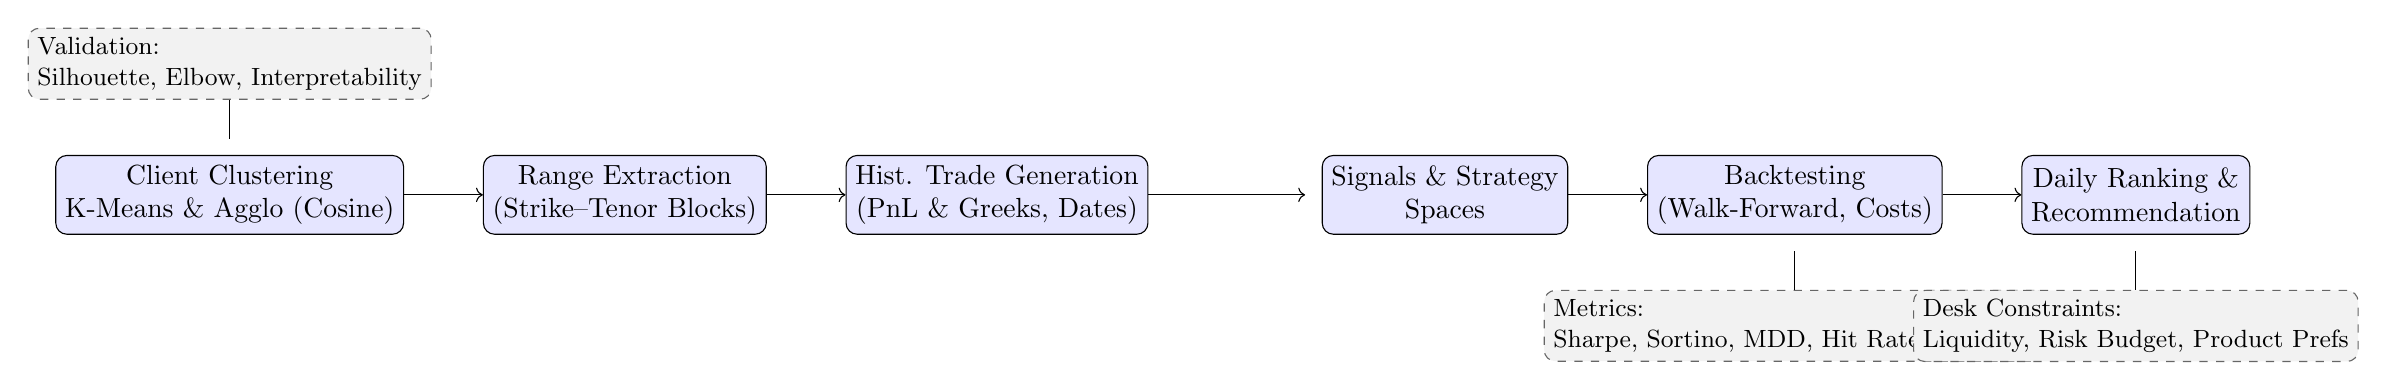
\begin{tikzpicture}[node distance=1cm]
\tikzstyle{box} = [rectangle, draw=black, rounded corners, minimum height=1cm, minimum width=1.7cm, align=center, fill=blue!10]
\tikzstyle{note} = [rectangle, draw=black!60, dashed, rounded corners, fill=gray!10, align=left, font=\small]

\node[box] (cluster) {Client Clustering\\K-Means \& Agglo (Cosine)};
\node[box, right=of cluster] (ranges) {Range Extraction\\(Strike--Tenor Blocks)};
\node[box, right=of ranges] (gen) {Hist. Trade Generation\\(PnL \& Greeks, Dates)};

\node[box, right=2.2cm of gen] (signals) {Signals \& Strategy\\Spaces};
\node[box, right=of signals] (bt) {Backtesting\\(Walk-Forward, Costs)};
\node[box, right=of bt] (reco) {Daily Ranking \&\\Recommendation};

\draw[->] (cluster) -- (ranges);
\draw[->] (ranges) -- (gen);

\draw[->, shorten >=6pt] (gen.east) -- ++(0.8,0) |- (signals.west);
\draw[->] (signals) -- (bt);
\draw[->] (bt) -- (reco);

\node[note, above=7mm of cluster] (val) {Validation:\\Silhouette, Elbow, Interpretability};
\draw[-] (val.south) -- ([yshift=2mm]cluster.north);

\node[note, below=7mm of bt] (metrics) {Metrics:\\Sharpe, Sortino, MDD, Hit Rate, Turnover};
\draw[-] (metrics.north) -- ([yshift=-2mm]bt.south);

\node[note, below=7mm of reco] (constraints) {Desk Constraints:\\Liquidity, Risk Budget, Product Prefs};
\draw[-] (constraints.north) -- ([yshift=-2mm]reco.south);
\end{tikzpicture}%
}
\caption{Two-part pipeline: client profiling (left) feeding the strategy \& recommendation engine (right).}
\label{fig:pipeline}
\end{figure}



\paragraph{Agglomerative clustering with cosine similarity.}
Beyond K-means, we use hierarchical agglomerative clustering to reveal a nested structure of client behaviors. Starting from singletons, clusters are merged iteratively until a single tree (dendrogram) is formed; cutting this tree at a chosen height produces the final groups.

\textbf{Dissimilarity.} We measure distances with \emph{cosine distance}
\[
d(\mathbf{x}_i,\mathbf{x}_j)=1-\frac{\mathbf{x}_i\cdot\mathbf{x}_j}{\lVert \mathbf{x}_i\rVert\,\lVert \mathbf{x}_j\rVert},
\]
so proximity reflects the \emph{composition} of strategy usage rather than absolute notional scale. Two clients with the same relative mix (e.g., bull vs.\ bear spreads) are close even if one trades larger size.

\textbf{Linkage.} To extend distance to clusters $C_p$ and $C_q$ we use \emph{average linkage}:
\[
d(C_p,C_q)=\frac{1}{|C_p||C_q|}\sum_{i\in C_p}\sum_{j\in C_q} d(\mathbf{x}_i,\mathbf{x}_j),
\]
a compromise between single linkage (chainy) and complete linkage (overly tight), yielding balanced groups.

\textbf{Procedure.}
\begin{enumerate}
  \item Initialize each client as its own cluster and compute the cosine-distance matrix.
  \item Repeatedly merge the pair of clusters with minimal $d(C_p,C_q)$, updating distances via average linkage.
  \item Stop when one cluster remains and \emph{cut the dendrogram} at a selected height to obtain the partition.
\end{enumerate}

\textbf{Example.} If $d(A,B)=0.2$ is minimal, merge $\{A,B\}$. Its distance to client $C$ becomes
\[
d(\{A,B\},C)=\tfrac{1}{2}\big(d(A,C)+d(B,C)\big).
\]
Choosing a cutoff, e.g.\ $d=0.4$ (at least $60\%$ cosine similarity), yields client groups with similar trading profiles.







% Ajouter la bibliographie au sommaire
\addcontentsline{toc}{chapter}{Bibliographie}

\bibliographystyle{plain}
\bibliography{references}   % Référence le fichier .bib (sans l'extension)


\end{document}